\documentclass[12pt letterpaper]{article}

\usepackage{fullpage}
\usepackage{graphicx}
\usepackage{amsmath}

\providecommand{\e}[1]{\ensuremath{\times 10^{#1}}}

\usepackage{float}


\title{Quantum Eraser Experiment}
\author{Johnny Minor \\ Partner: Kayla Mitchell}
\date{\today}

\begin{document}

\maketitle

%abstract should have a very brief overiew of the goals and main results of the experiment. 
\begin{abstract}
In this set of experiments we used a red laser through a wire various polarizer configurations which resulted in unique patterns that could be seen on a viewing screen. Based upon the configuration of polarizers the laser would sometimes create an interference pattern. While other times it would not. When it would not create an interference pattern was when we had information about which side of the wire the laser came through. This information was created by placing polarizers in different configurations on each side of the wire. This fact might lead classical thinking to believe that the wave function had collapsed to a possibility, and would continue to stay that way. However, when we introduced a polarizer after we knew which side the photons had came through we recovered the interference pattern. Therefore, we have found in this experiment that in classical thinking it might seem that we have altered the history of the photons. Of course this isn't the case because we're not time travelers, and it is only a matter that the information of the wave function can manifest itself in either way and only depends on what you force it to be. In other words the wave function doesn't collapse completely until we observe or detect it.   
\end{abstract}

\newpage

\section*{Description of Experiment}

It is a well known result from Quantum Mechanics that the double slit experiment will yield an interference pattern. This was first studied by Thomas Young in the early 1800s. We know now that this behavior is due to the dual nature of photons. They can manifest themselves as a particle or a wave. Which nature they manifest is based on how they are being measured at that time. However, we are interested not in a simple double slit but what happens when we force the photon to exhibit its particle nature, but then destroy that information. We are interested if the photons will then continue to be particles, or if they will suddenly exhibit wave nature again. In our experiment we studied this dualistic behavior. We experimented with how we can first make photons exhibit particle like behavior and then change the experiment slightly to make them to appear to exhibit wave like nature. 

In order to study this behavior we used a 635 nm red diode laser. Importantly we began by finding the which direction the polarization of the laser was. To do this began by directing the laser at a piece of plexiglass. We then varied the angle of the plexiglass  while noting the intensity of the reflected light on the wall next to us. We varied the the angle of plexiglass from about 30 degrees to 140 degrees. As we varied the angle we could see the the intensity of light get lighter and then increase again. Due to this result we concluded that red diode laser was "p" polarized. We know that "p" polarization exhibits this nature because we saw the intensity decrease and then increase again. We can clearly see this from the figure \ref{fig:s_and_p} that with p type polarization when we vary the angle of incidence we see a decrease in the reflectance. 

%from http://cvilaseroptics.com/support/Technical-Library/Optical-Coatings
\begin{figure}[!ht]
  \caption{s and p polarization from: http://cvilaseroptics.com/support/Technical-Library/Optical-Coatings  }
  \centering
    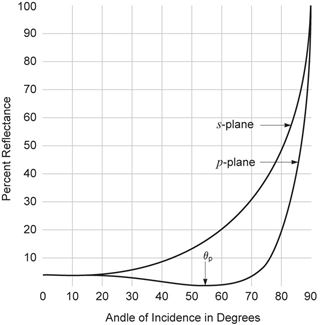
\includegraphics[width=.5\textwidth]{s_and_p_polarization.jpg}
    \label{fig:s_and_p}
\end{figure}

Since the laser was linearly polarized we were forced to place a polarizer at approximately 45 degrees behind the output of the laser (in other words the laser will go through the 45 degree polarizer sheet). This was needed to force the photons to be polarized at about 45 degrees. This meant that since the photons were polarized at 45 degrees they will have two vector components. This is important because later on we would want to put our 45 degree light through a vertical polarizer and a horizontal polarizer. If, for instance, we had only the horizontally polarized light and then put it through a vertical polarizer we would get nothing out. Since the light was polarized at 45 degrees we could put the light through both a vertical polarizer and a horizontal polarizer. It is important to try to get the polarizer at 45 degrees otherwise one component will have  a greater magnitude and that would lead to issues with the interference. 

So the setup for our experiment was as follows:
\begin{figure}[!ht]
  \caption{The quantum eraser experiment setup.}
  \centering
    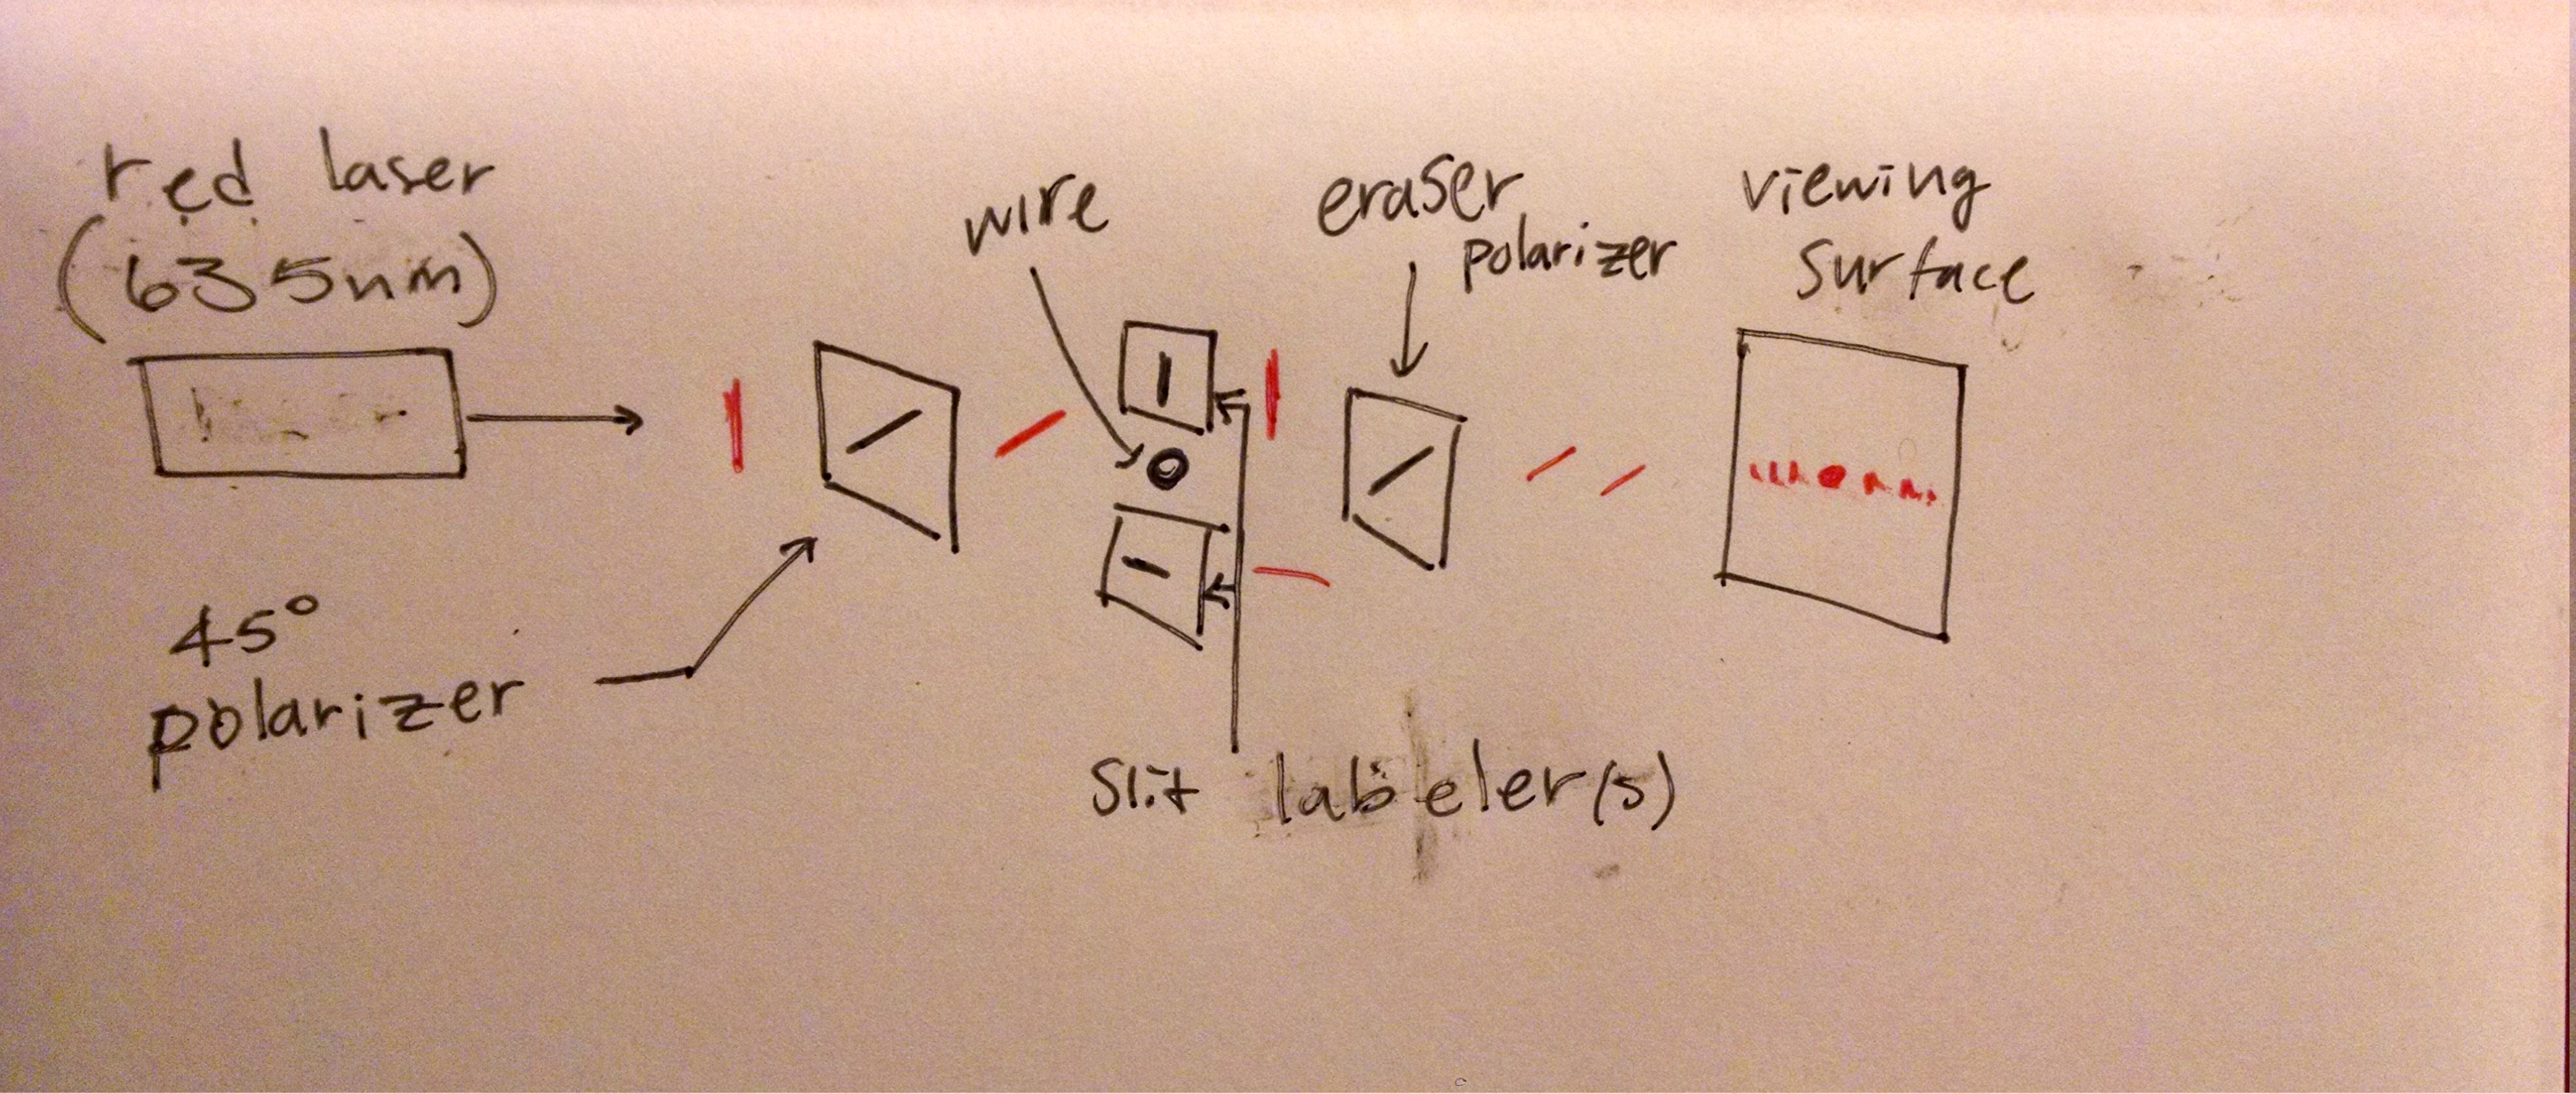
\includegraphics[width=.75\textwidth]{quantum_eraser_setup.jpg}
    \label{fig:setup}
\end{figure}

From here, since we knew which direction the laser was polarized, we were able to orient the polarizer vertically. We did this because the wire that we were going to use was oriented vertically too. this would enable us to see the interference pattern easier. 

We also used two sheets of polarizer material with their polarizations placed orthogonal to one another and put the later through them. We observed that the interference patter went away. 

We also placed polarizers behind the path labeler(the path labeler is another name for the two orthogonal sheets of polarization placed on each side of the wire) in both vertical and horizontal positions. This yielded two different blobs of light. 

Finally, we moved the polarizer from vertical to 45 degrees clockwise and counterclockwise from vertical. We noted that the interference pattern returned.  
  

 

%\begin{figure}[!ht]
%  \caption{The double slit setup}
%  \centering
%    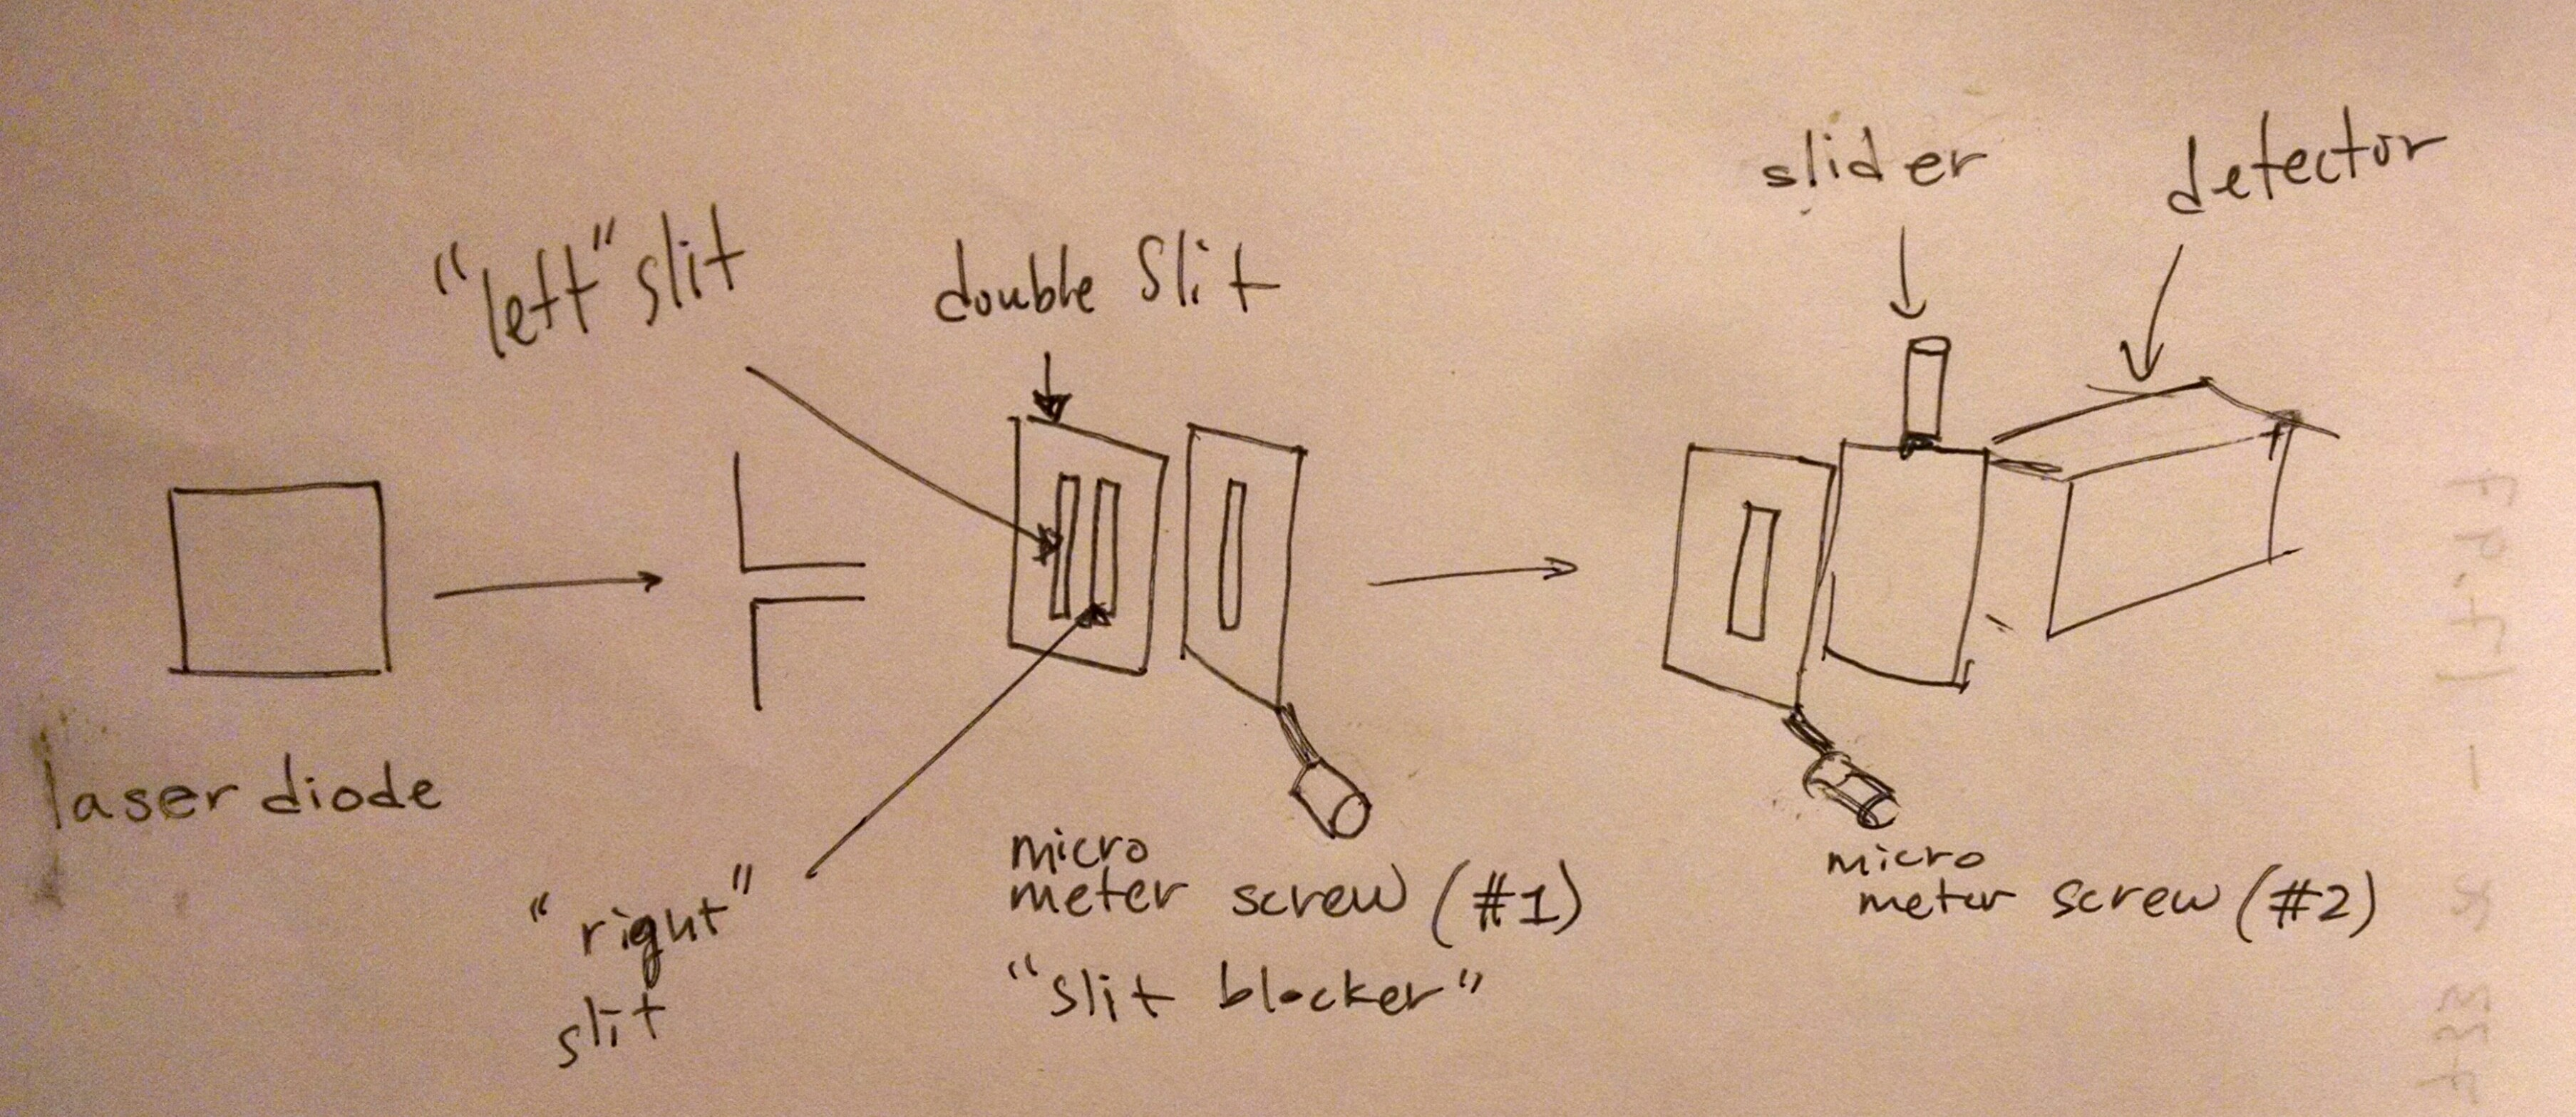
\includegraphics[width=\textwidth]{double_slit_setup.jpg}
%    \label{fig:double_slit_setup}
%\end{figure}




\section*{Data and Analysis}

In our first experiment we aimed our linearly polarized laser at a polarizer that was turned 45 degrees counter clockwise from vertical. This resulted in an interference pattern that can be seen in figure \ref{fig:interference}. This interference pattern can be thought of using classical electromagnetic theory by the photons waves interfering once being split by the wire. The waves will then interfere with each other both constructive and destructively. Where they constructively interfere is where we see spots of greater intensity and spots of no intensity is where there is destructive interfere. This experiment could also be thought about using Quantum Mechanics. With Quantum Mechanics the photon is a discrete particle with an associated wave function. The wave function's absolute value squared yields a probability distribution. So, quantum mechanically we can reason that we see the interference pattern because this is the probability distribution of the particle. In other words, we see the highest concentration of particles at the central peak because that is where they are most likely to be. The photon has zero probability at the points where we see no intensity of light. 

\begin{figure}[H]
  \caption{The interference pattern from the wire}
  \centering
    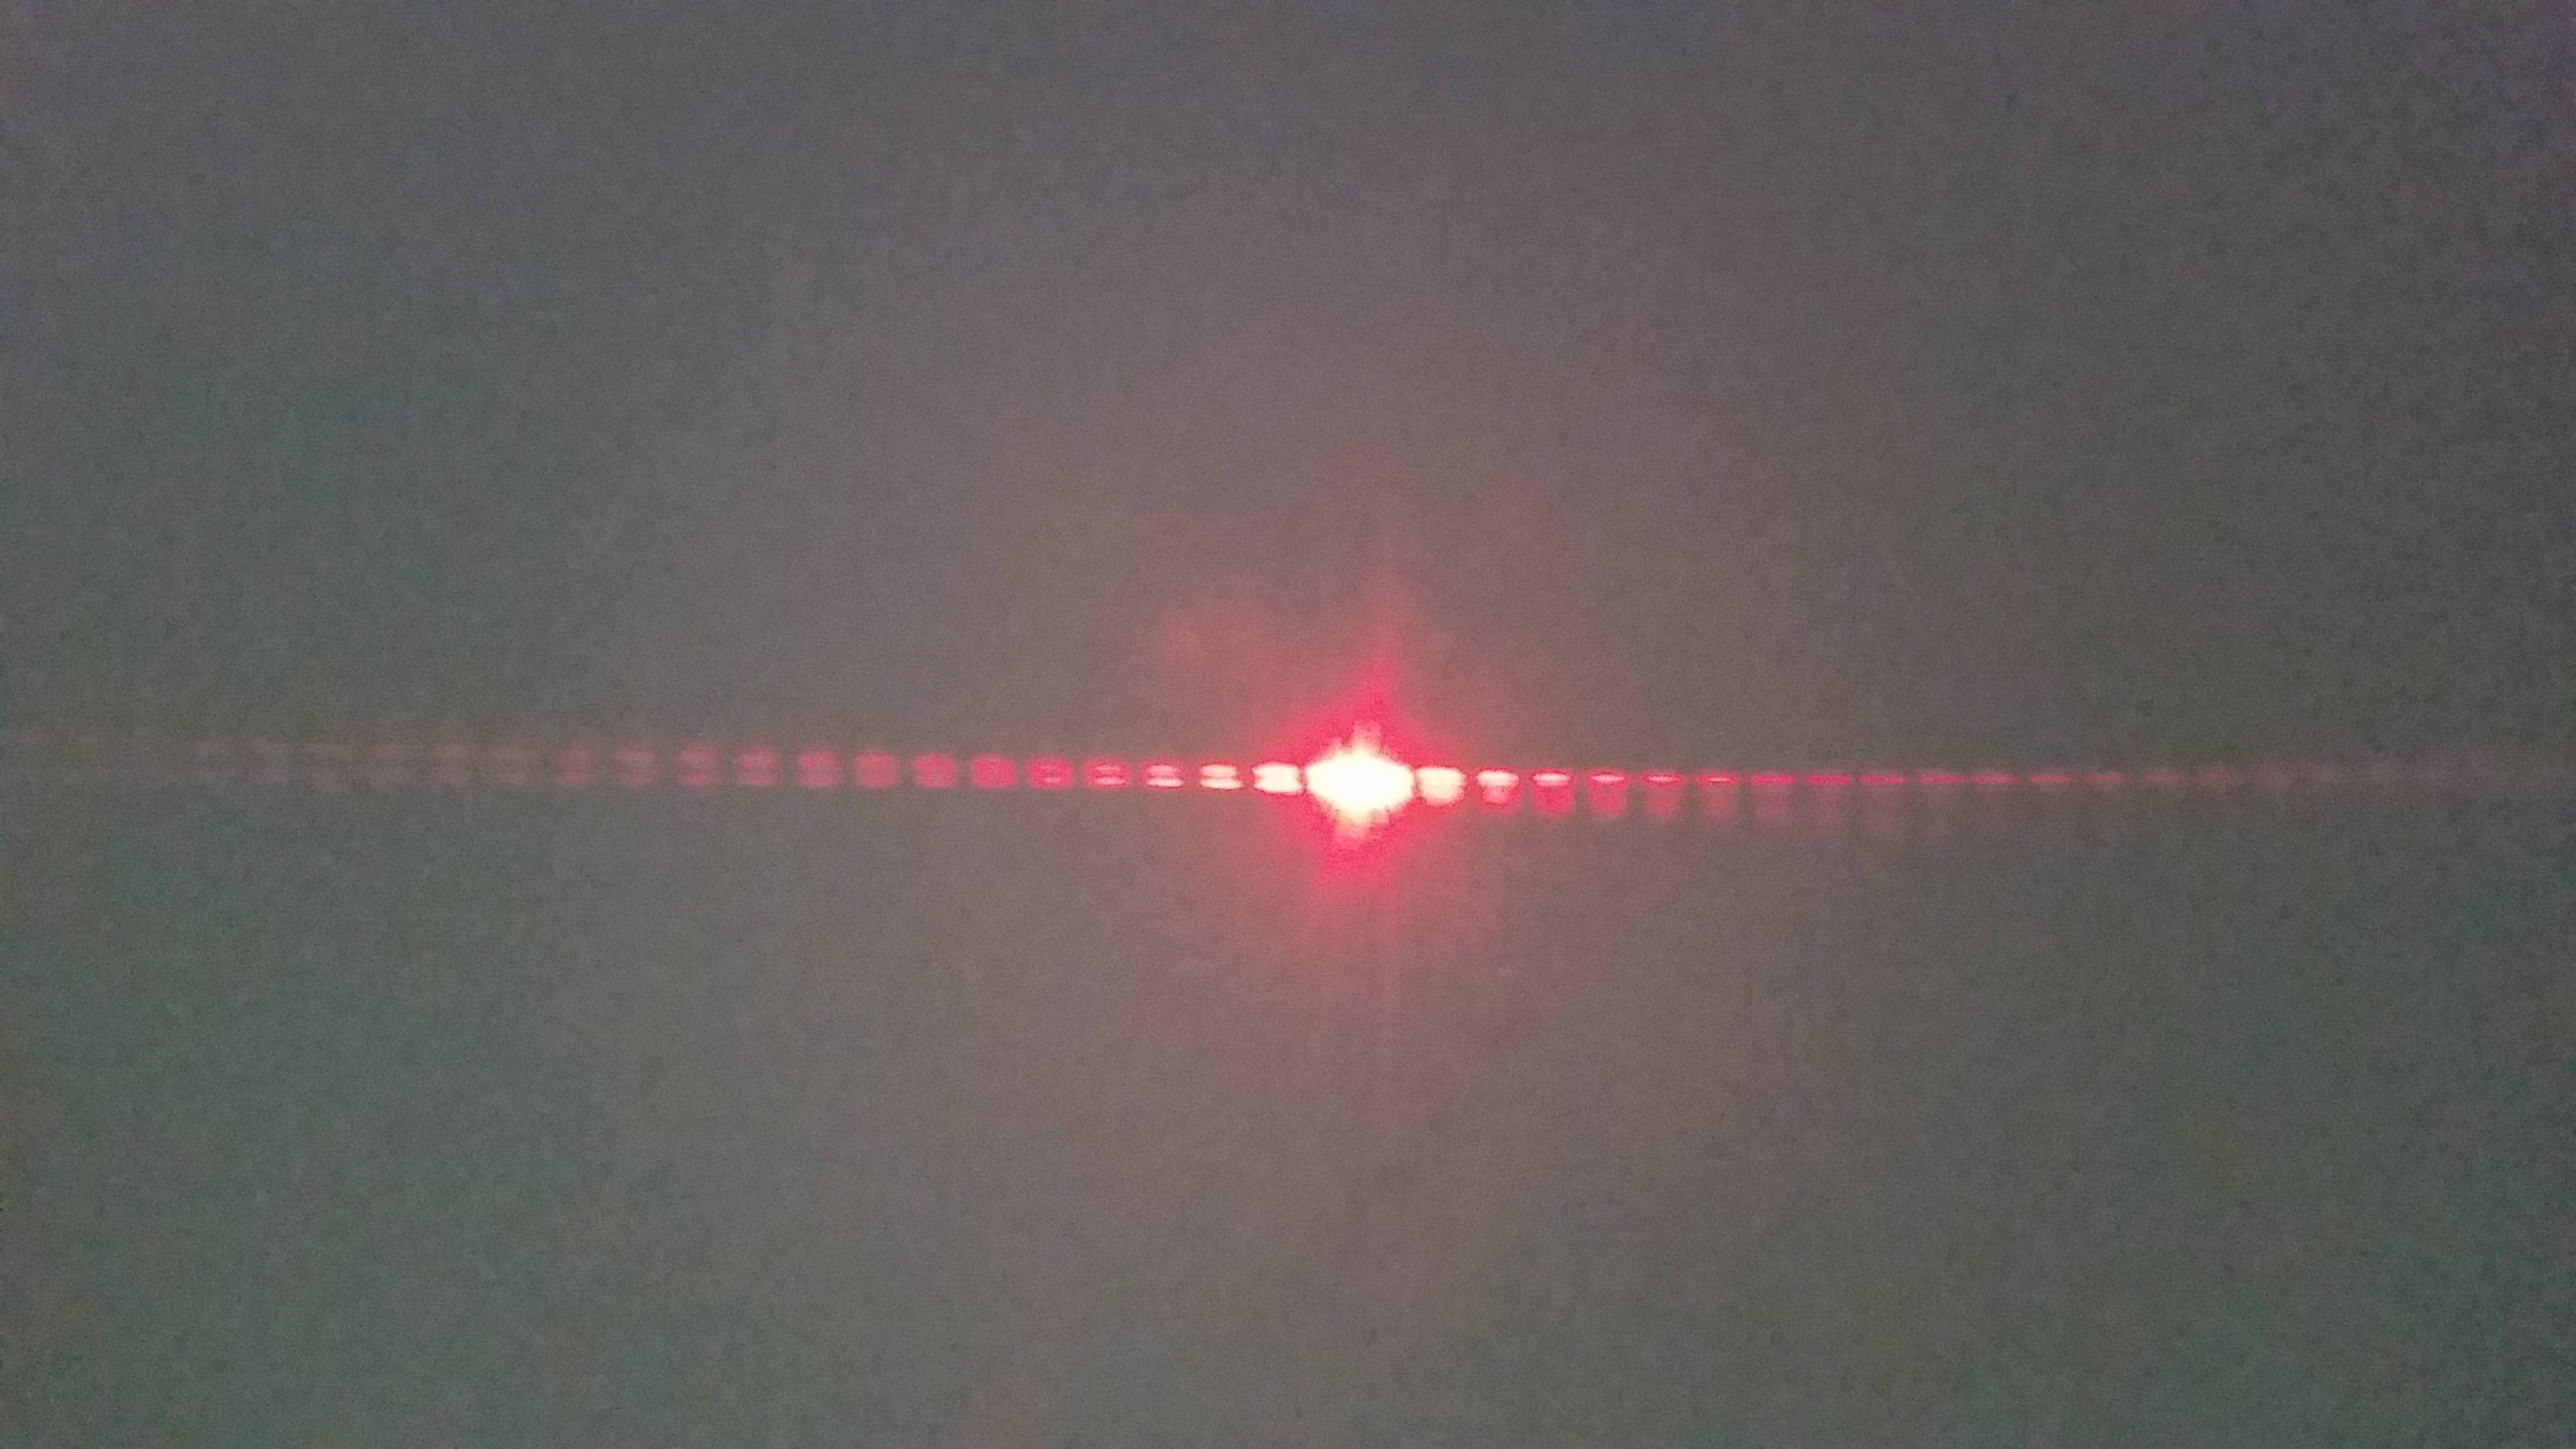
\includegraphics[width=.75\textwidth]{interference.jpg}
    \label{fig:interference}
\end{figure}

In our second experiment we placed two sheets of polarized material that were orthogonal to each other next to the wire. What this means is that on one side of the wire the polarizers transmission axis was vertical, and on the other side of the wire the polarizers transmission axis was horizontal. This meant that we gained information on which side the of the wire the photon traveled because if a photon went through the side with the polarizer that was vertical then we \textit{know} it went through that side, and alternatively the same for the horizontally oriented polarizer. Because of this we have gained information about the system. So, we saw the interference pattern disappear.  

This can be explained using electromagnetism by saying that the electromagnetic wave will break apart into two parts as the wave goes through the two polarizers. This leads to a blob of intensity. In quantum mechanics we can say that since we have information about which path the photon took we then made the wave function collapse to a certain position. This position is most probable at the point that we observed in figure \ref{fig:path_label}  

\begin{figure}[H]
  \caption{The pattern from the path labeler}
  \centering
    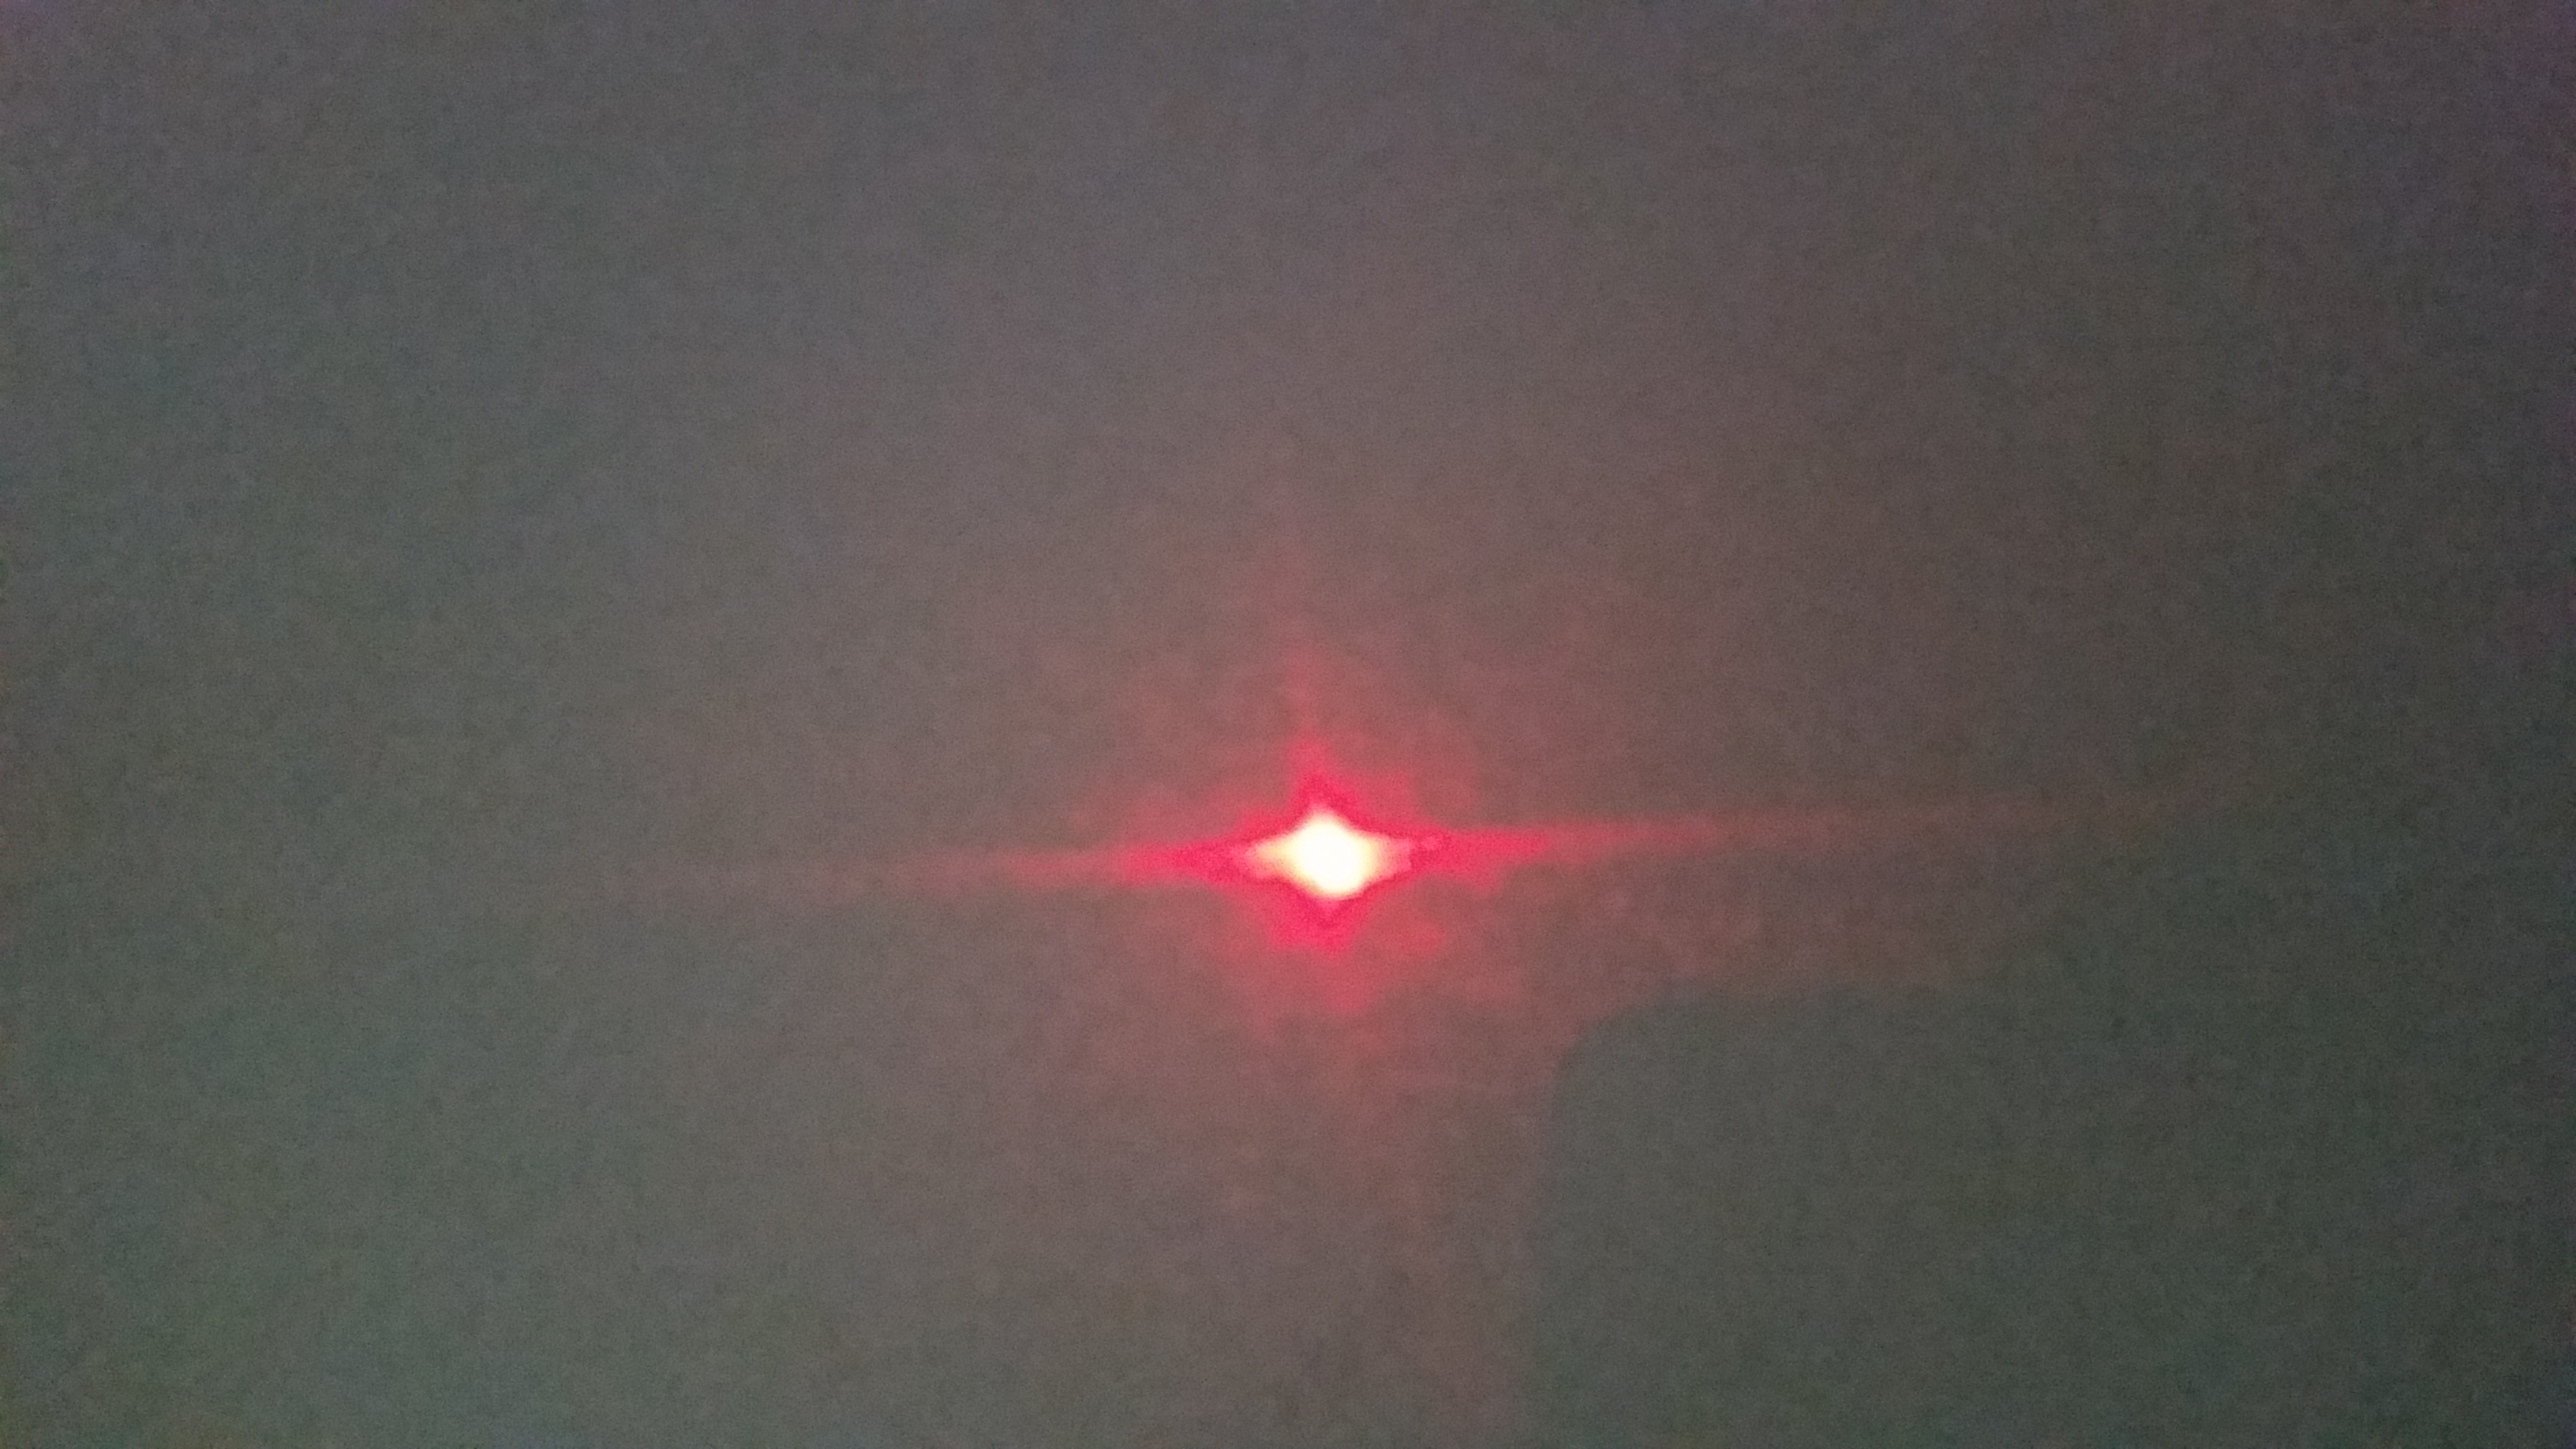
\includegraphics[width=.75\textwidth]{pathlabel.jpg}
    \label{fig:path_label}
\end{figure}

In our third experiment we placed a polarizer with a vertically oriented transmission axis behind the path labeler that we used in our second experiment. This meant that we would only see the photons that went through one side of the path labeler because only one side had vertically polarized light coming through it. This new polarizer would block the horizontally polarized light because that light is orthogonal to the transmission axis. This resulted in a single spot of intensity. We then oriented a polarizer horizontally and we see nearly the same result. These two results can be seen in figure \ref{fig:left photons} and in figure \ref{fig:right photons}. 

We can think about this result using classical Electromagnetic theory. The electromagnetic wave will get through both vertically oriented polarizers and finally be seen on the viewing screen, but the light that is polarized orthogonal(horizontal) to the second polarizer will be blocked. We can also think about this using Quantum Mechanics. If we treat a photon as a single particle then the we can think of it as having a probability of going through each slit. The probability of it making through the horizontally oriented polarizer and then the vertically oriented polarizer is zero. So we don't see any intensity of light. However, there is great probability of it going through both vertical polarizers and therefore we see the spot of intensity. 

\begin{figure}[H]
  \caption{The left passing photons.}
  \centering
    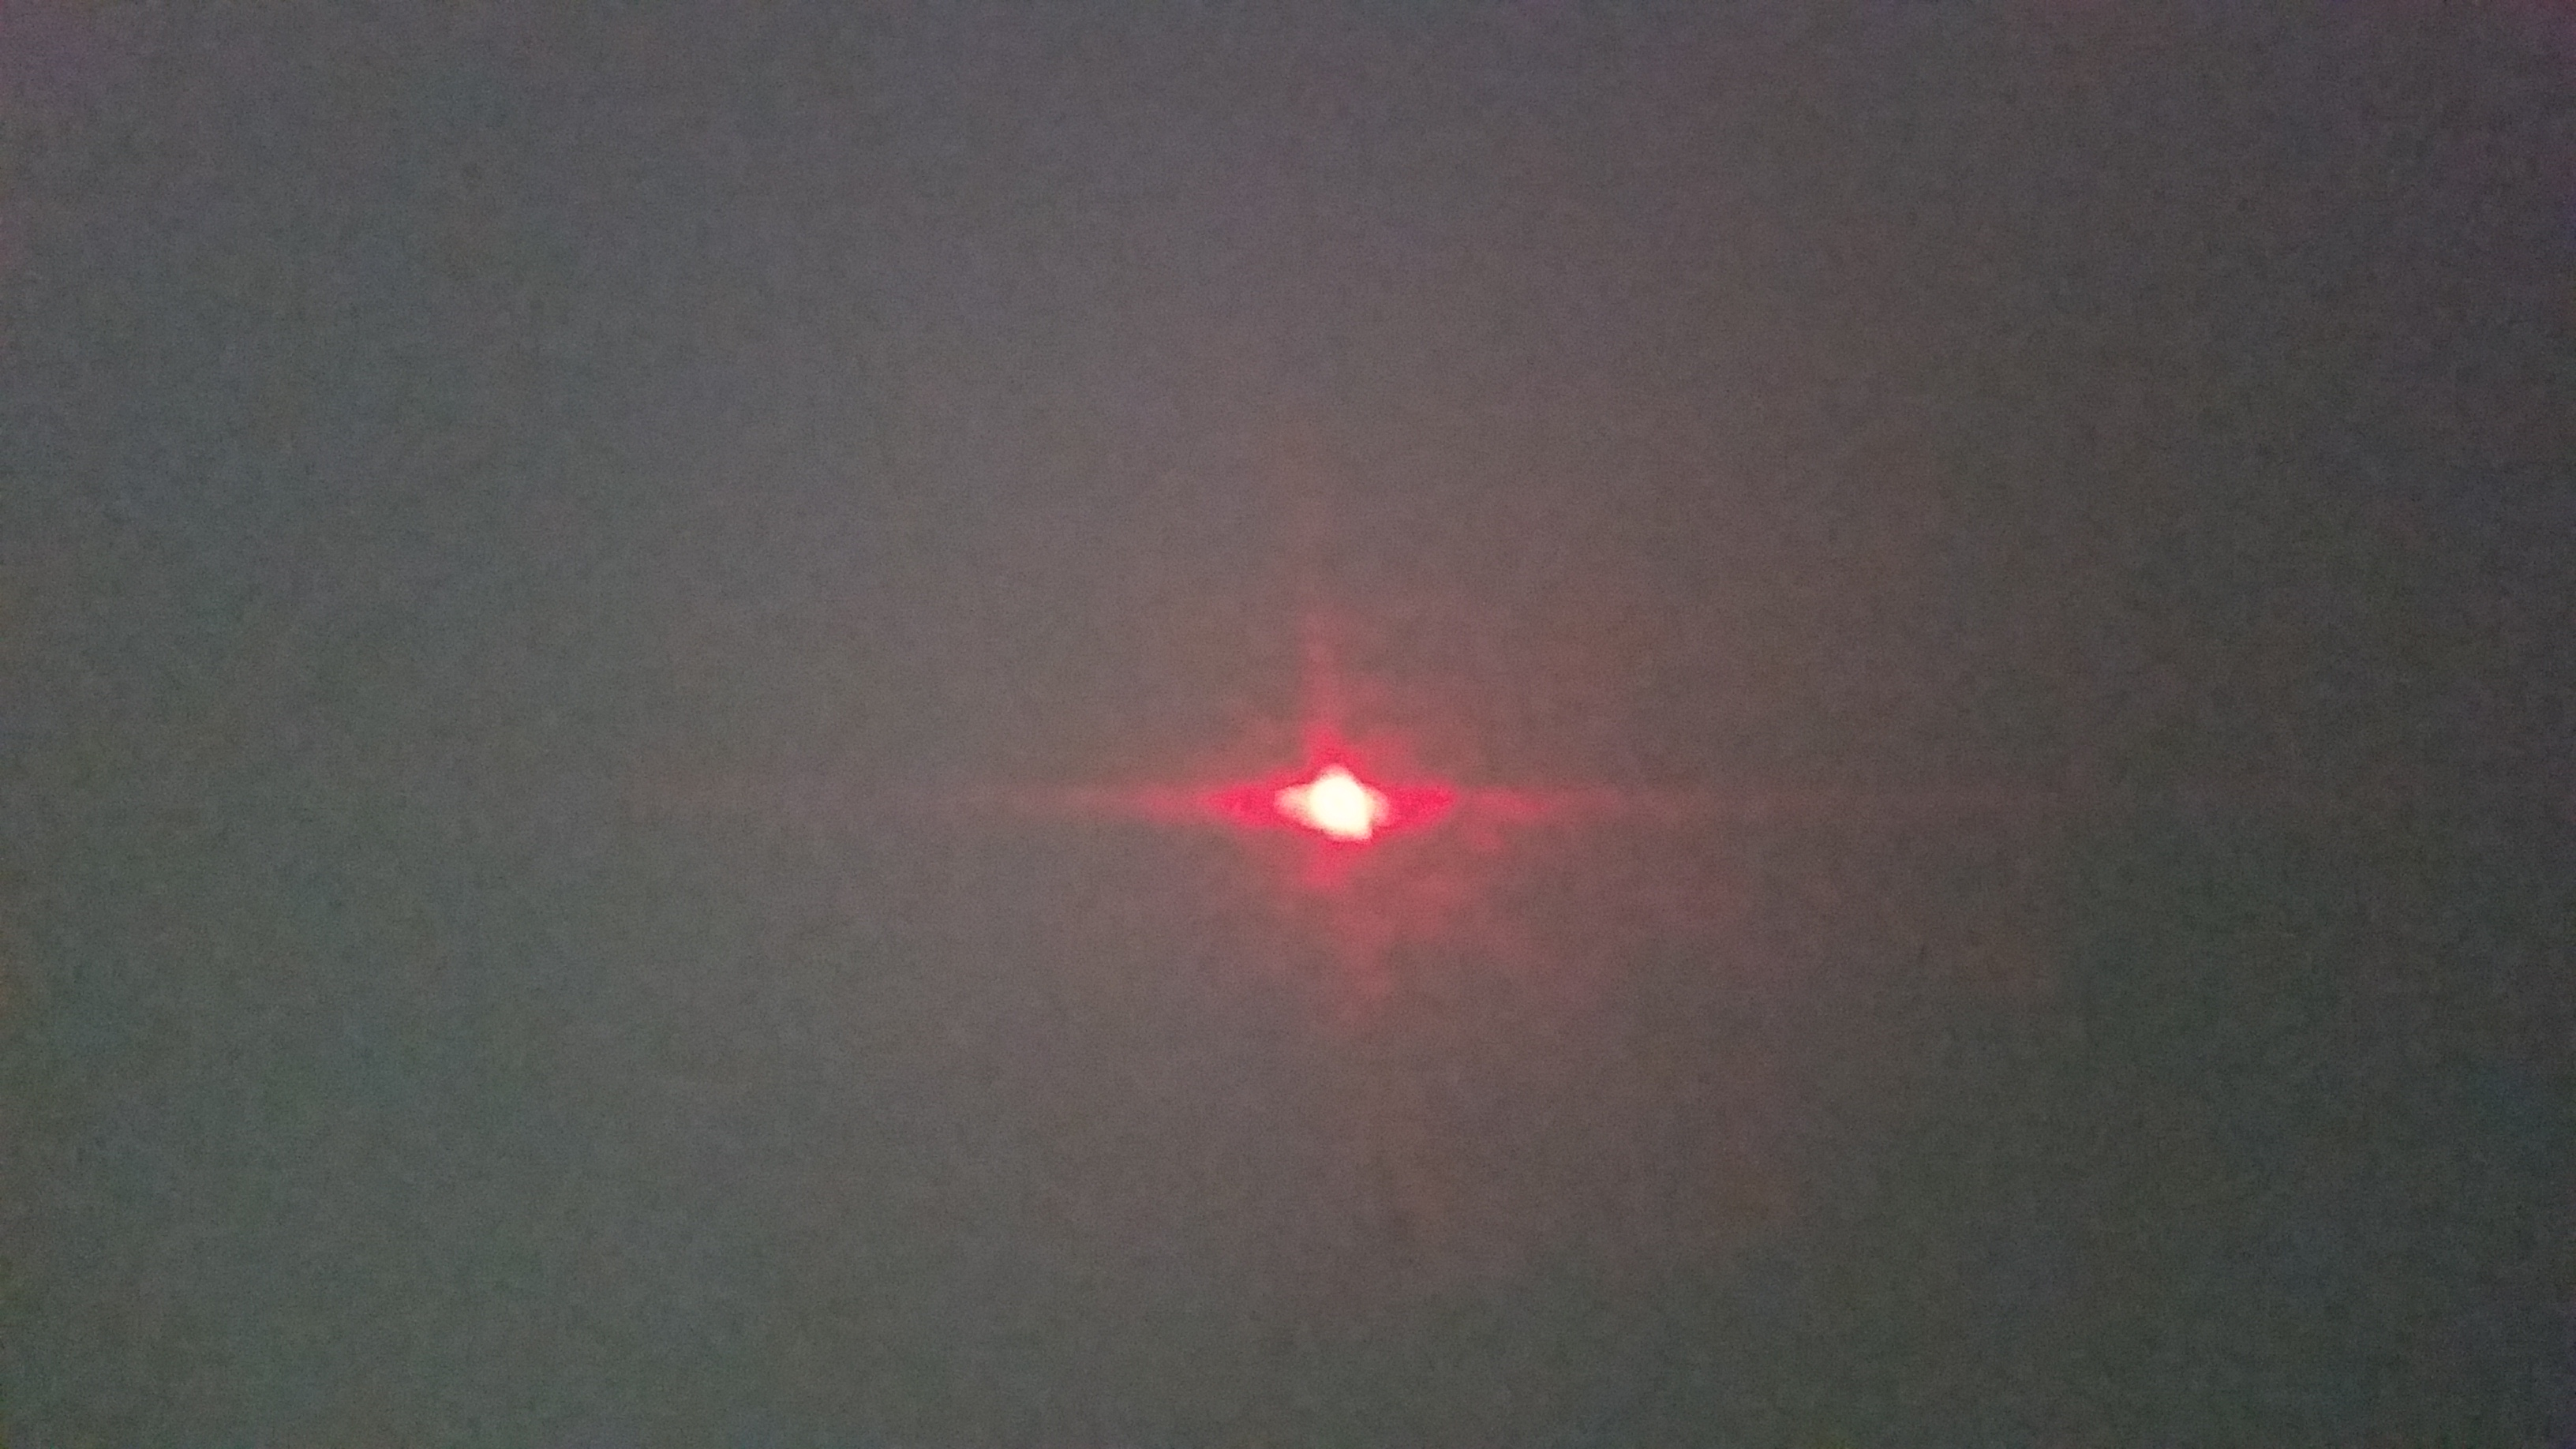
\includegraphics[width=.75\textwidth]{left_photons.jpg}
    \label{fig:left photons}
\end{figure}

\begin{figure}[H]
  \caption{The right passing photons.}
  \centering
    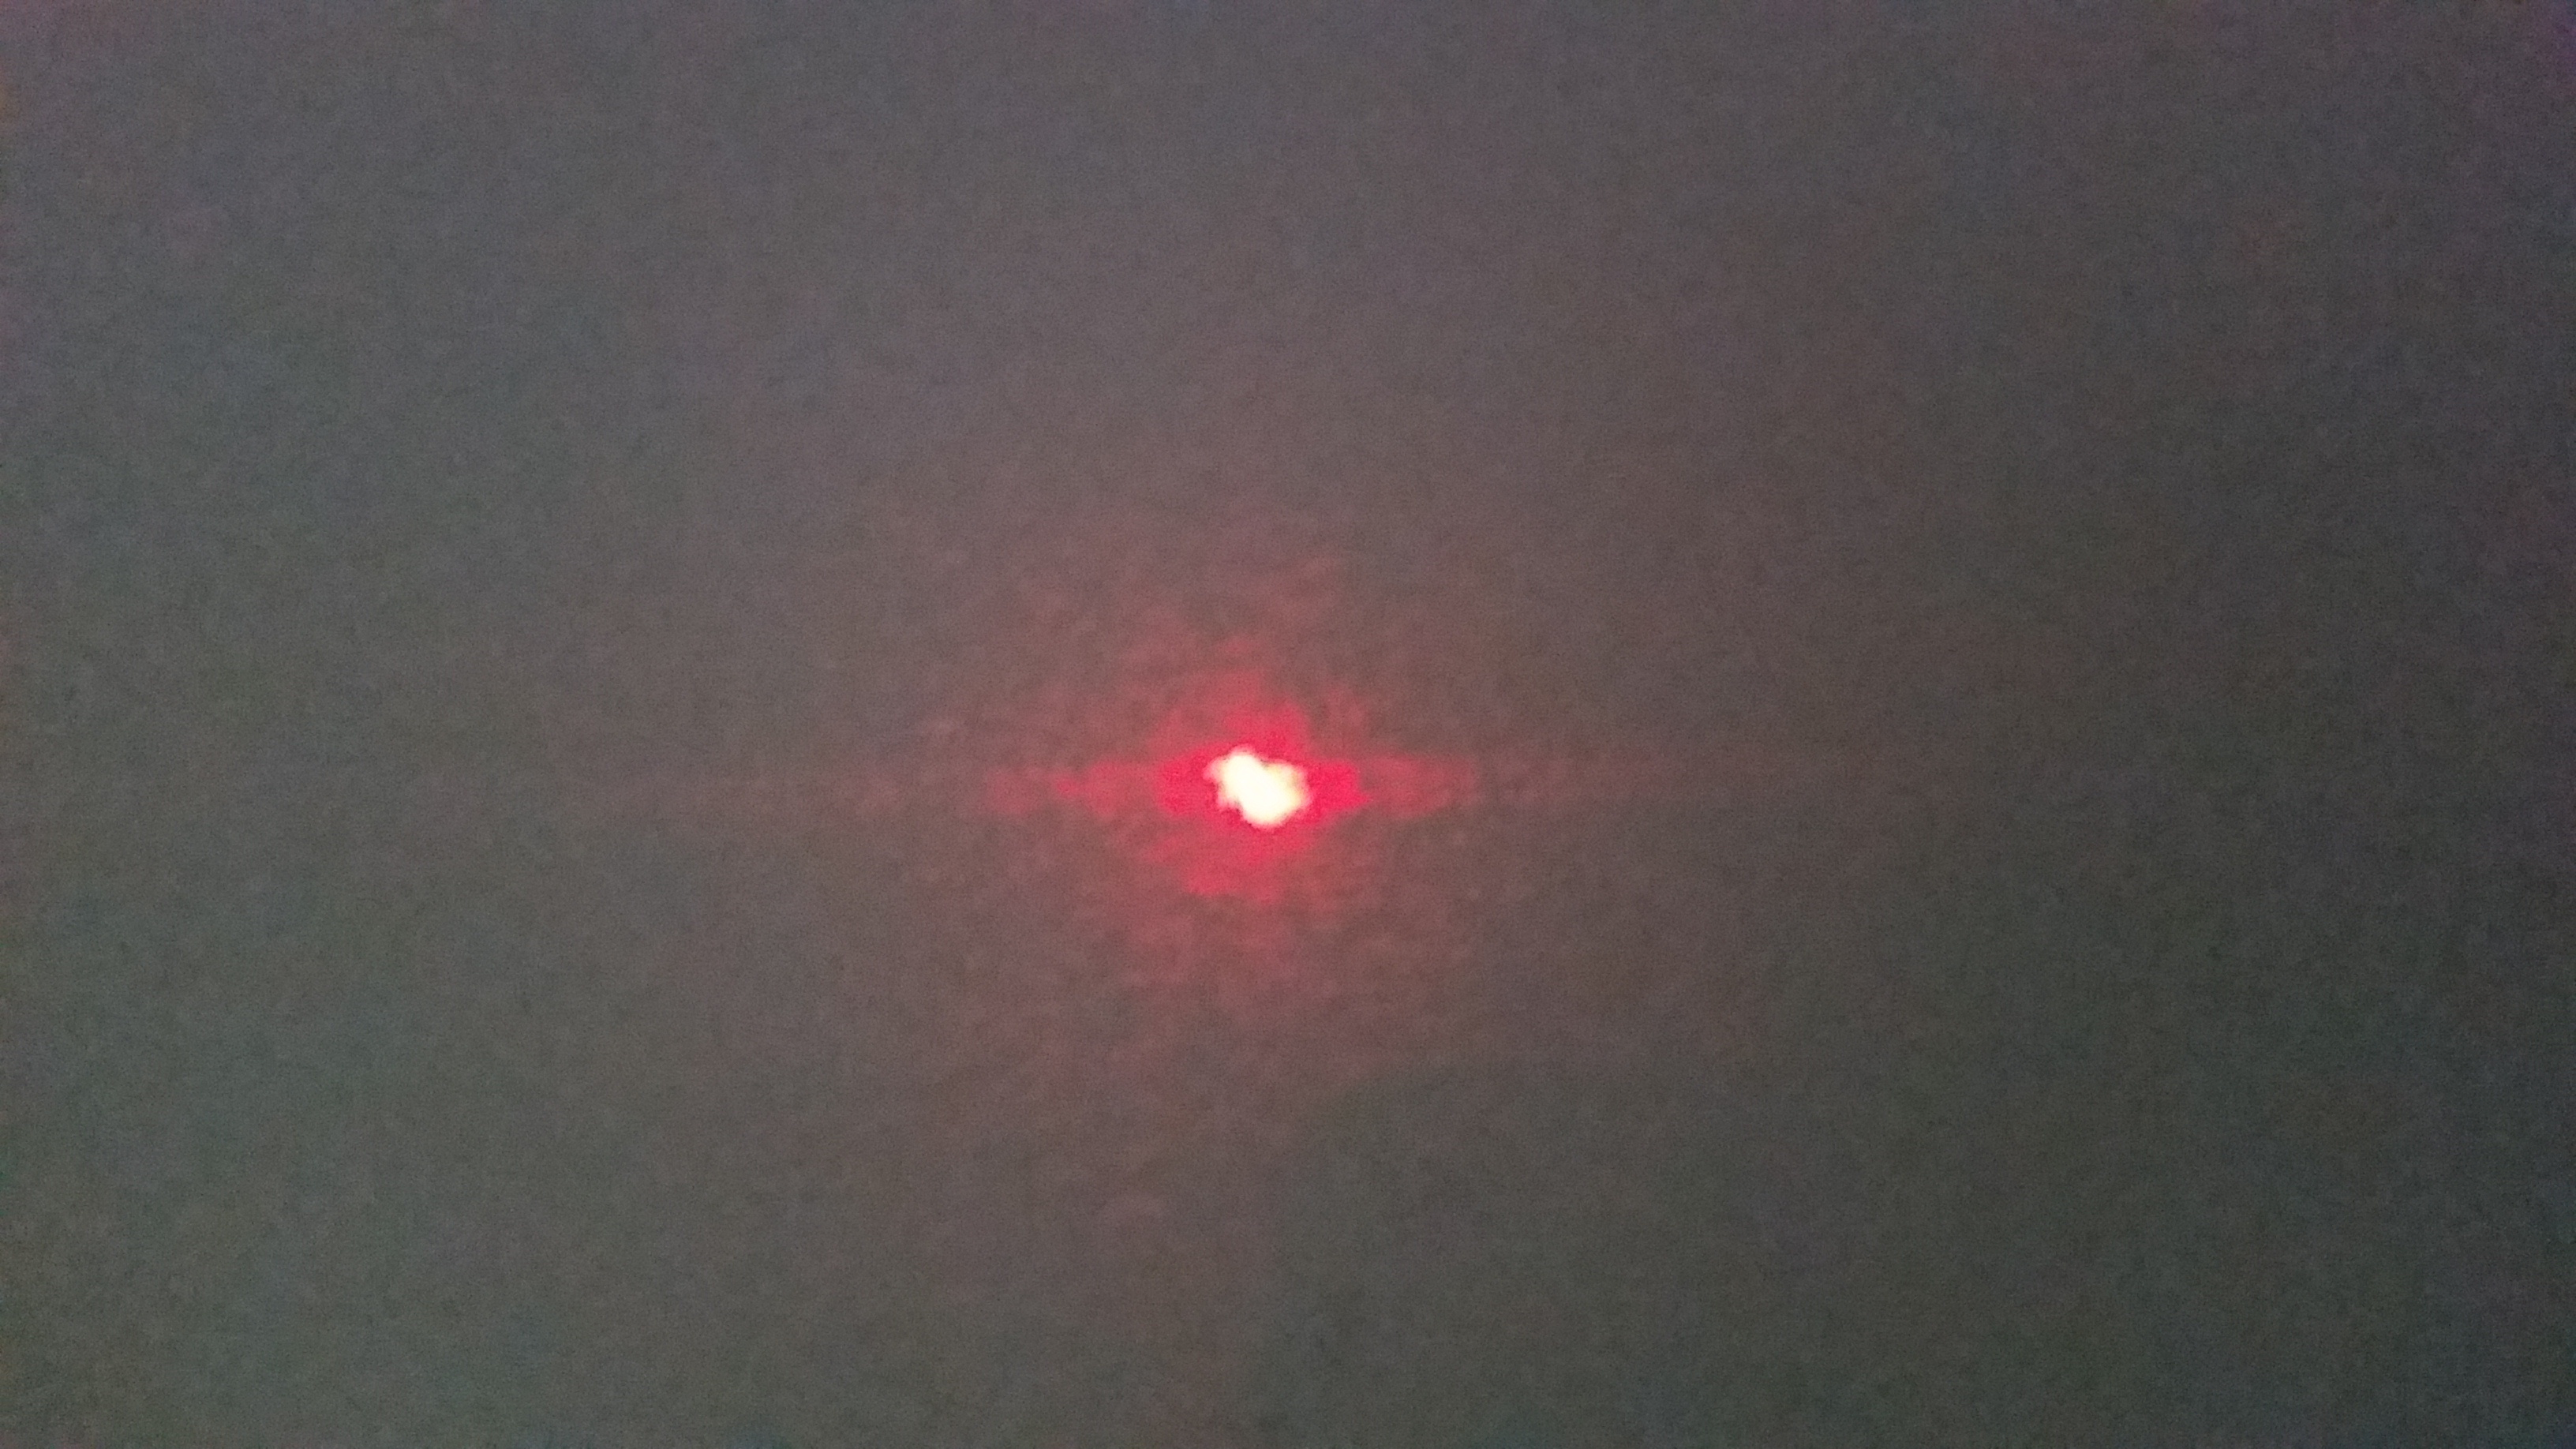
\includegraphics[width=.75\textwidth]{right_photons.jpg}
    \label{fig:right photons}
\end{figure}

In our fifth experiment we placed a polarizer at 45 degrees from clockwise and counterclockwise (two separate experiments) behind the slit labeler. This created an interference pattern in both instances. These can clearly be seen in figure \ref{fig:erased1} and figure \ref{fig:erased2}. When we add the polarizer we erased the path information because we get a contribution from both the horizontally and vertically polarized light. This then means that they can interfere once again. 

If we treat this experiment this classic Electromagnetic theory then we can justify this result by reasoning that the vertically polarized photons and the horizontally polarized photons will only add their components to the the 45 degree polarizer. This will then lead to interference. If we treat this result using Quantum Mechanics we can say that since the the photon has equal probability of going through either the vertical or horizontal polarizer and then it has probability of going through the 45 degree polarizer that the wave function has a corresponding probability that results in having a higher probability at the center and then zero probability at the dark spots. 


\begin{figure}[H]
  \caption{The pattern from a polarizer at 45 degrees from vertical counter clockwise behind the wire.}
  \centering
    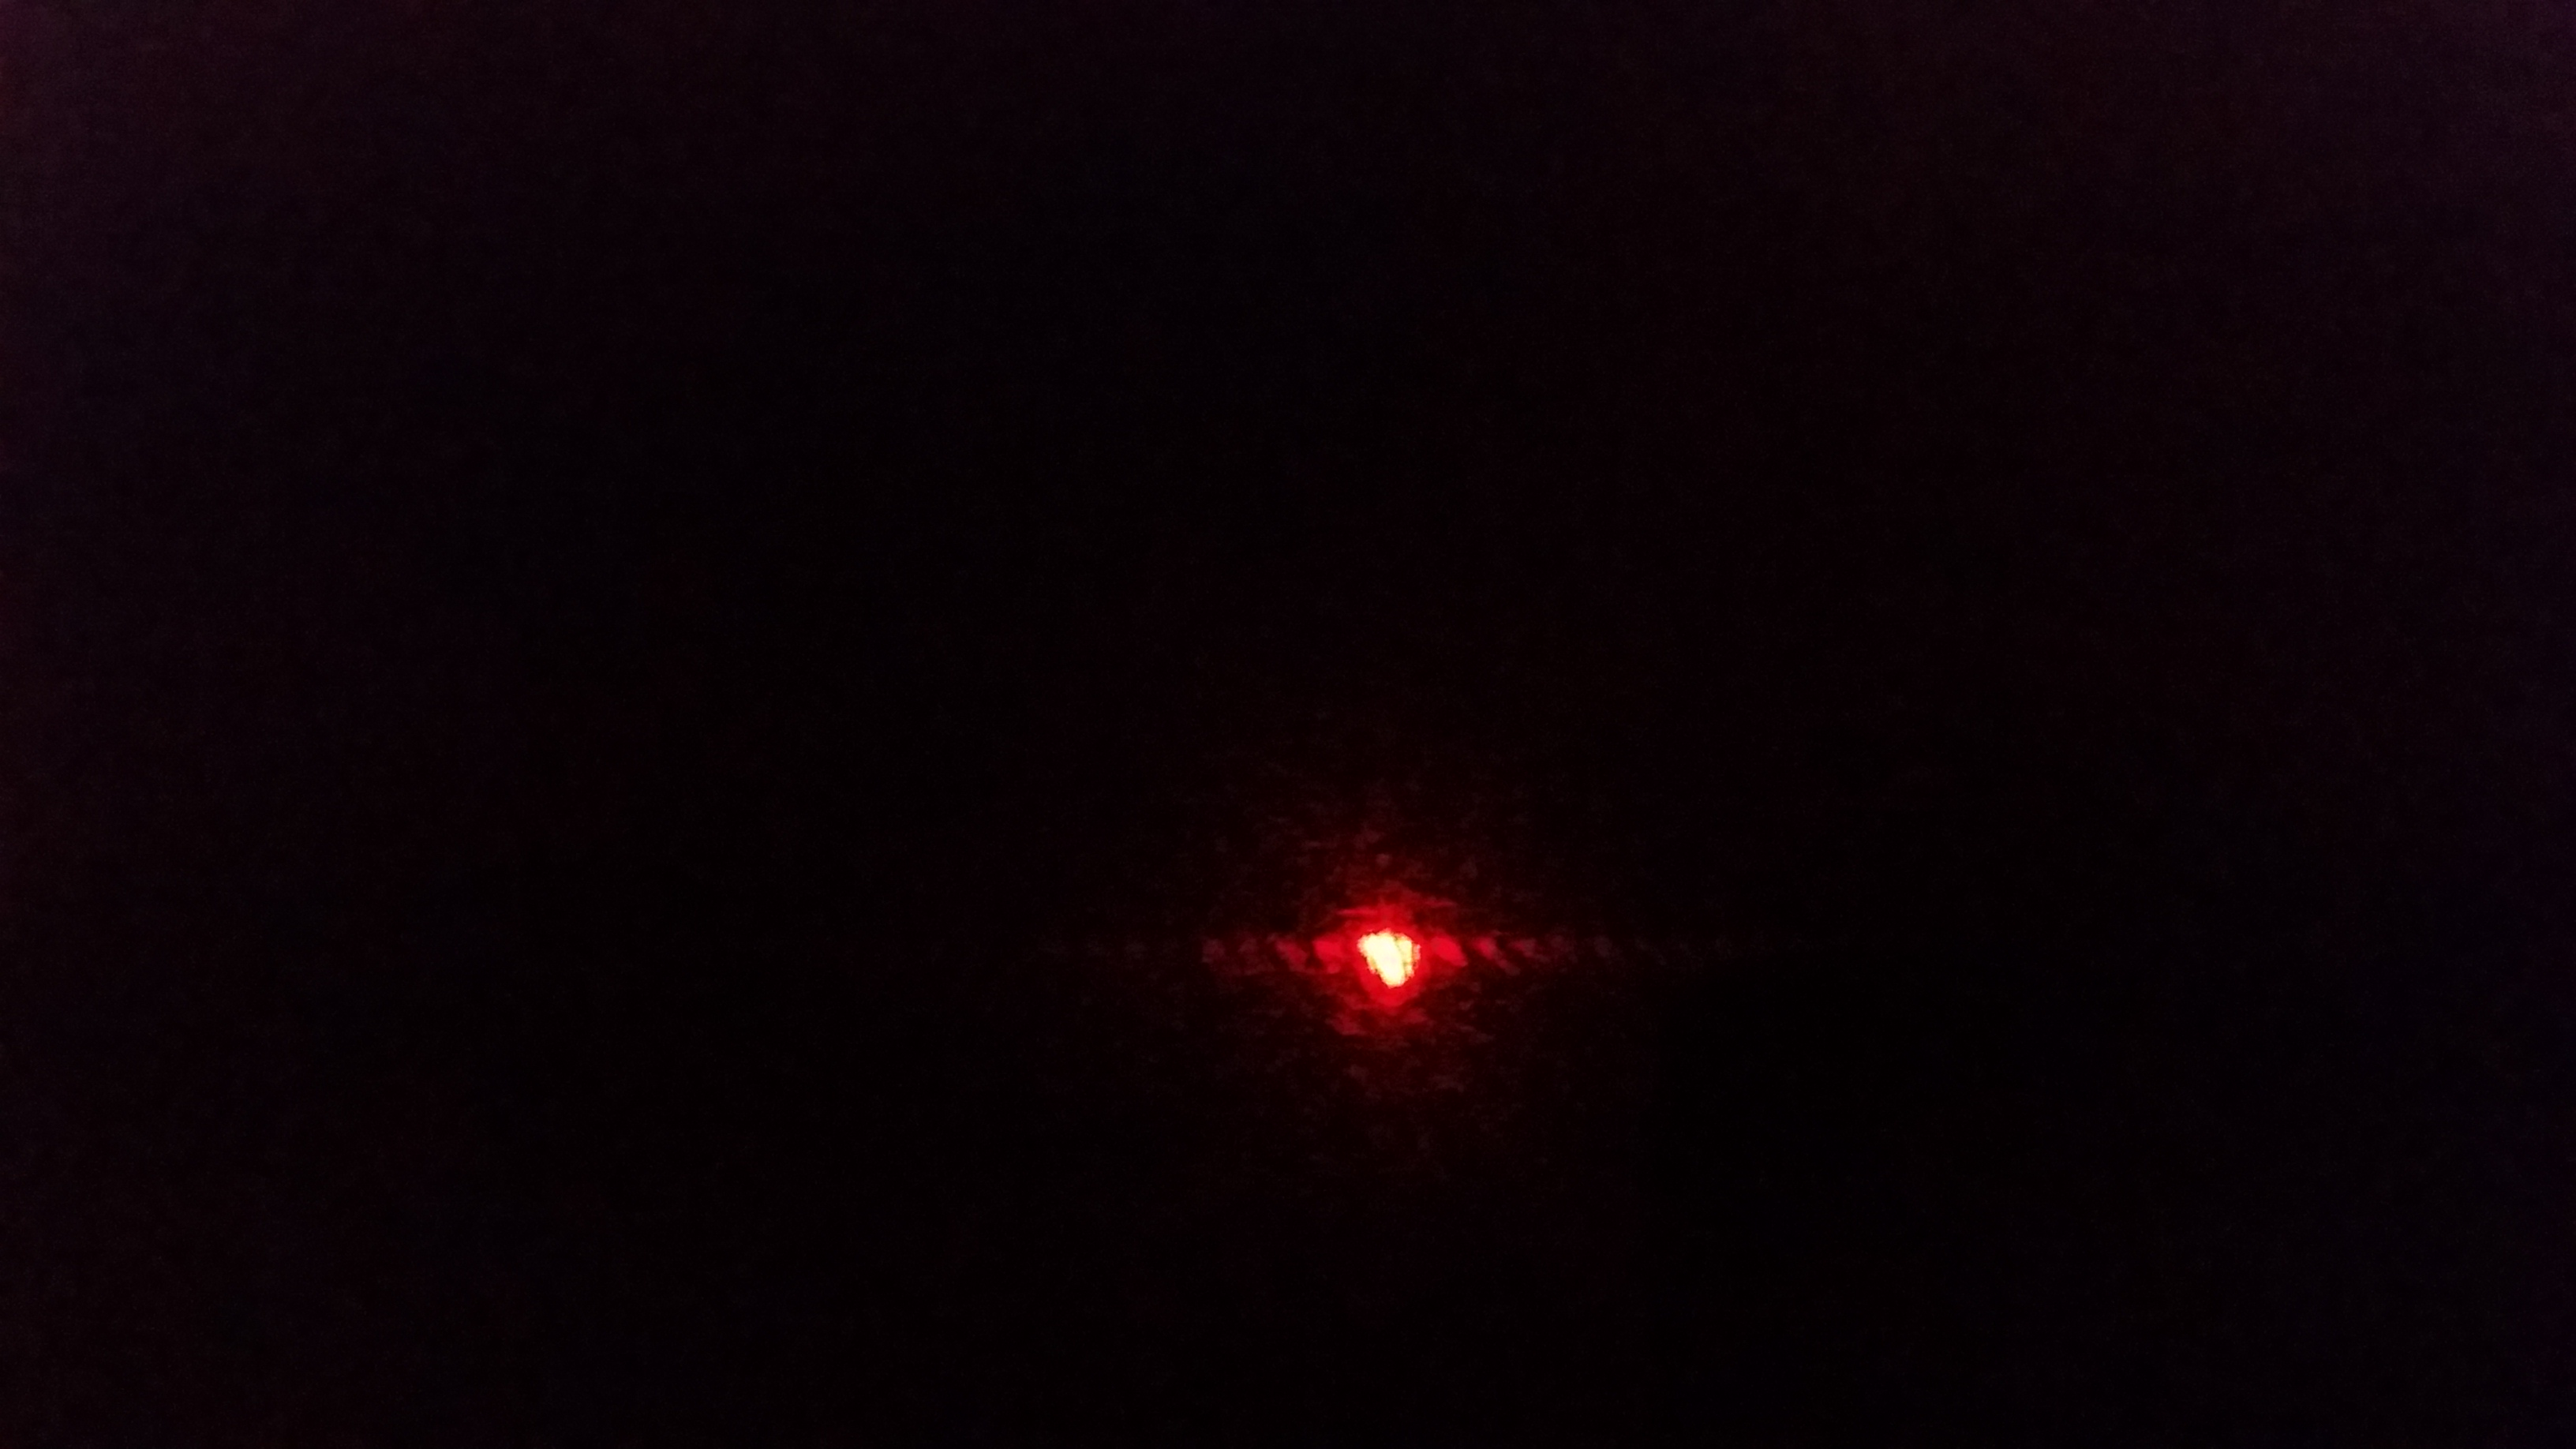
\includegraphics[width=.75\textwidth]{erased1.jpg}
    \label{fig:erased1}
\end{figure}

\begin{figure}[H]
  \caption{The pattern from a polarizer at 45 degrees from vertical clockwise behind the wire.}
  \centering
    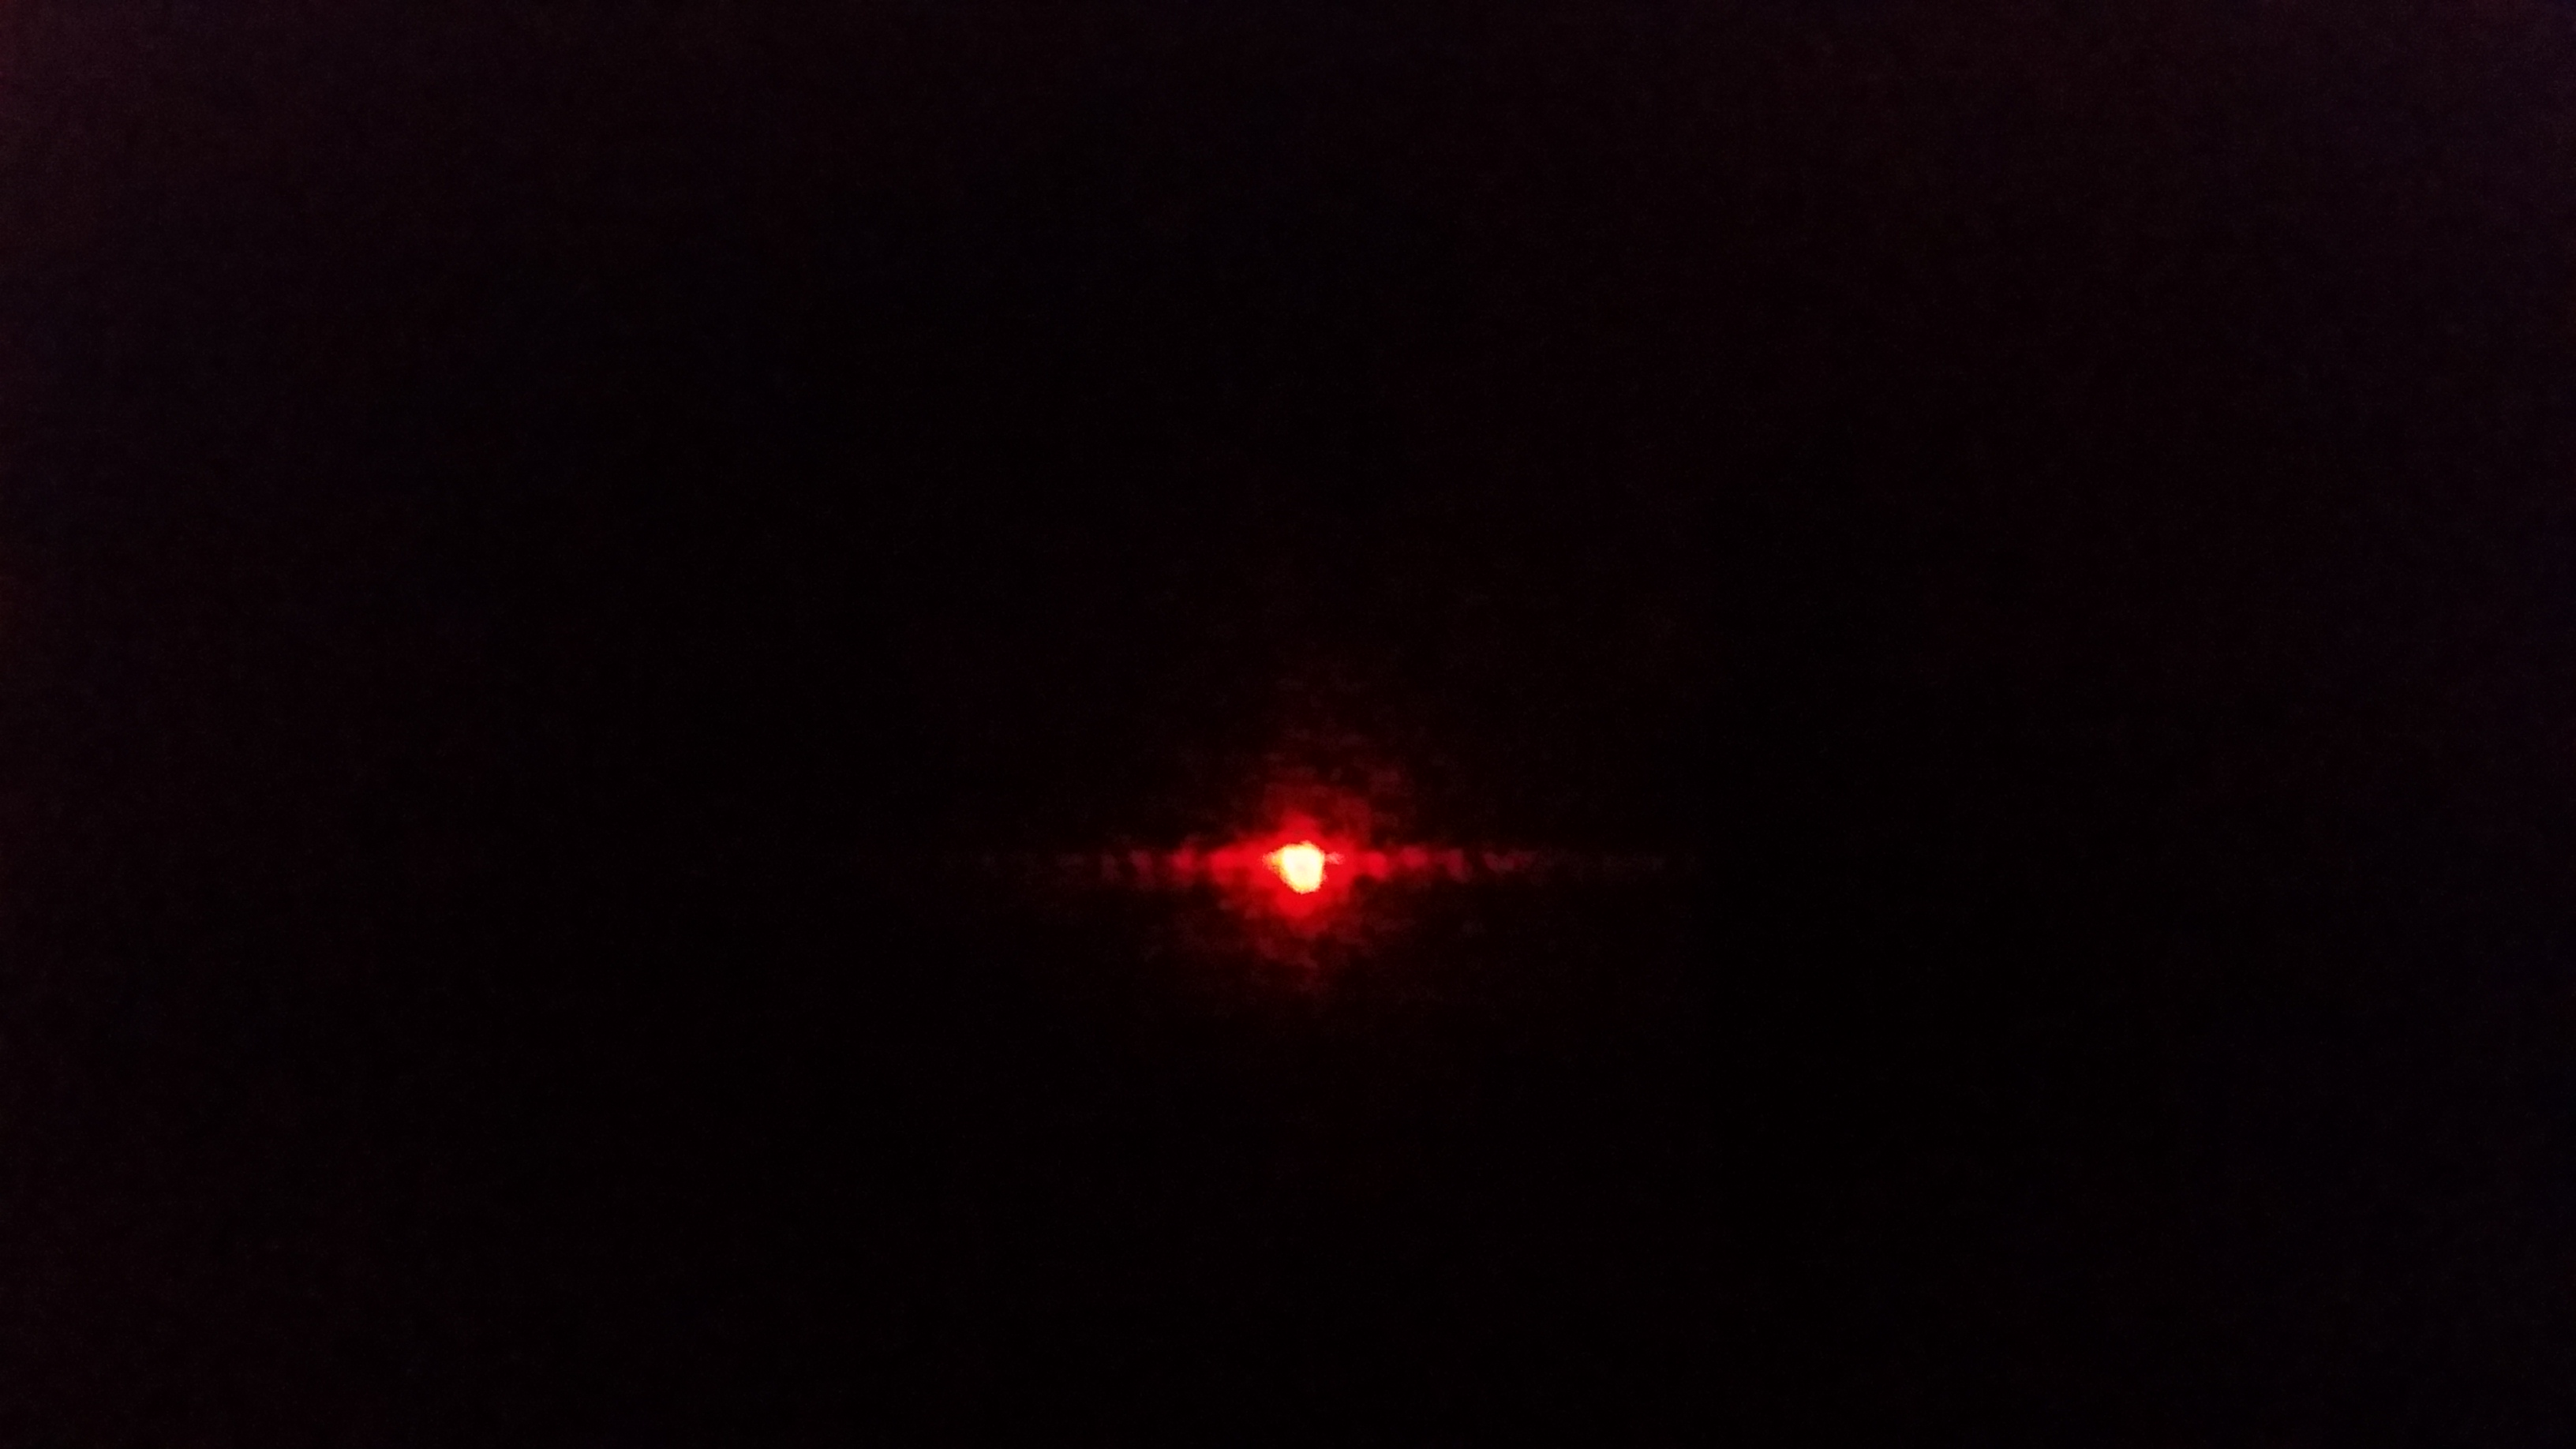
\includegraphics[width=.75\textwidth]{erased2.jpg}
    \label{fig:erased2}
\end{figure}

In our final experiment we placed a "hybrid eraser" behind the wire. The hybrid eraser is a two triangular polarizer sheets that had been taped together. The top piece had its polarization axis 45 degrees from clockwise. While the bottom piece had its axis of polarization 45 degrees counter clockwise. This resulted in two interference patterns that were orthogonal to each other. We observed the interference pattern in figure \ref{fig:hybrid}. 

We can think about this using classic Electromagnetic theory by thinking that the polarized waves go through both the top half and bottom half. When they do they create an interference pattern. Using Quantum Mechanics we can think about the photons as particles that will having a probability distribution that corresponds to the interference pattern. The photons will have a probability of going through the top polarizer or the bottom and then the wave function will collapse and create the interference pattern. 


\begin{figure}[H]
  \caption{The pattern from a hybrid eraser behind the wire.}
  \centering
    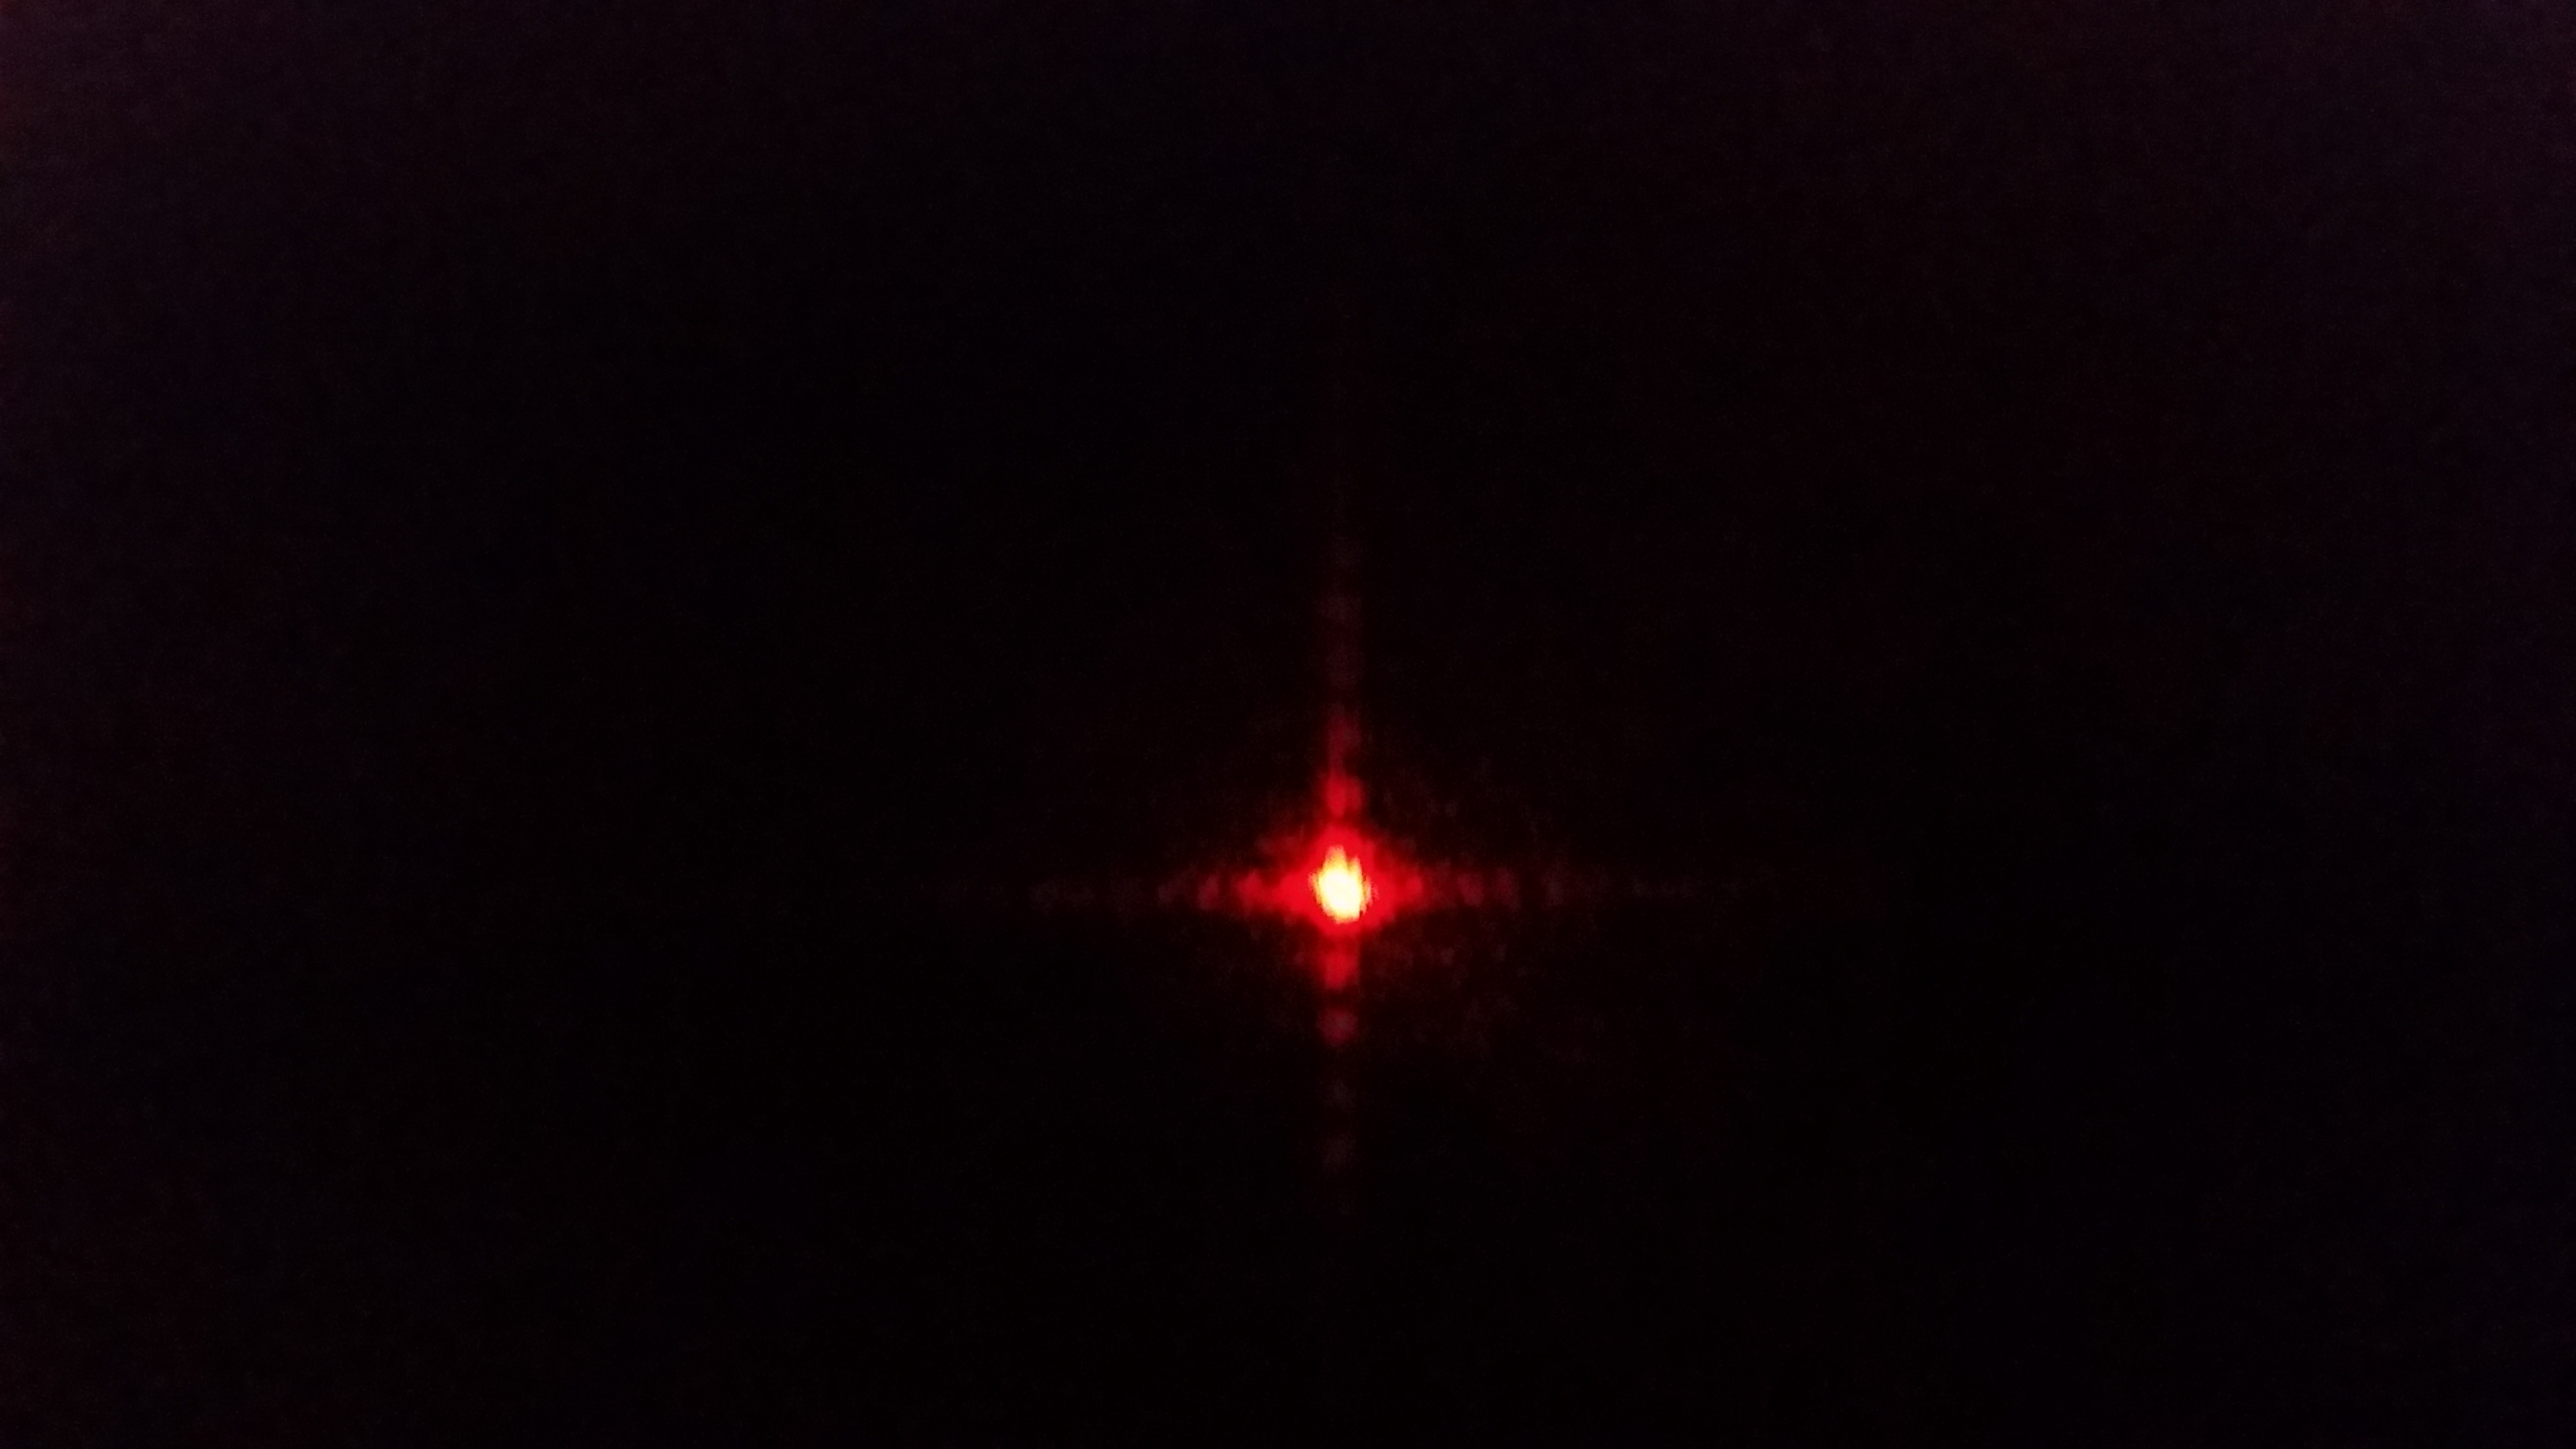
\includegraphics[width=.75\textwidth]{hybrid_eraser.jpg}
    \label{fig:hybrid}
\end{figure}



\section*{Results and Conclusions}

In this experiment we have shown the truly peculiar nature of Quantum Mechanics. We have shown that we can measure things in the future that seem to effect what happened in the past. This manifested itself in our experiment by showing that when we have information on which side of the wire the light went the interference pattern would go away and all we would see is a blob of light. When we destroyed ("erased") this information with our 45 degree polarizer the pattern would appear. It would seem that removing our information recovered the interference pattern. This experiment has confirmed the wave-particle duality of the photon in Quantum Mechanics. 

However, this experiment is not purely ``quantum". As we described how this can be explained using classical Electromagnetic theory in each part of Data \& Analysis section. In order for this experiment to be truly quantum we would need to only shoot a single photon through the experiment. Thus, we would be only sending a single "quanta" of light through the apparatus. However, a single photon wouldn't be enough. We would really need to send hundreds or perhaps thousands of photons through the apparatus before we began to make out a pattern. This pattern would be the probability distribution of the wave function, or theoretically speaking the absolute value squared of the wave function. If we conducted our experiment in this manner then it would truly be considered quantum, but the experiment would yield the same result. 
(\textit{Question 10})

We're not entirely sure how to interpret the result that it seems as if we're changing the past. We would hypothesize that we are not travelers of time. Instead we are merely getting information from the photon by the measurement that we place on it. It would seem that all of the information of the photon is available it is just a matter of what information we force the wave function to return. In other words all the information contained in the wave function is there until we measure the photon. 
(\textit{Question 11}) 

We measured the diameter of the wire that we were aiming our red laser at with a pair of calipers that were provided. We found the diameter to be 0.24 mm. Using our understanding of Fraunhofer diffraction we can model our interference pattern as slit single. We can find the width of the slit, or wire in our case. Employing the small angle approximation because our angle or very small because our viewing surface is much further away in distance than the width of our single slit (or diameter of wire). So, we measured the distance from the wire to the wall and found it to be approximately 18 feet. We measured the distance from the central peak to the next central peak to be 7.90 mm. As we see in figure \ref{fig:fraunhofer} the Faunhofer equation 
\begin{equation}
\label{eq:fraunhofer}
y \approx \frac{m \lambda D}{a}
\end{equation}

where $y$ is the distance from peak to peak, m is the node number, $\lambda$ is the wavelength of light, and $a$ is the slit width. So re can rearrange equation \ref{eq:fraunhofer} to solve for $a$. We can then plug our values in to solve for $a$. We found $a$ to be 0.196 mm. This value is only 0.044 mm different than the value we measured with the calipers. Such a small error could come from our measuring the distance from the wire to the viewing surface, our measurement from peak to peak, or not having exactly a 635 nm red laser. It would seem most likely that our error comes from inaccuracies in our measurements. 


\begin{figure}[H]
  \caption{The Fraunhofer equation from: http://hyperphysics.phy-astr.gsu.edu/hbase/phyopt/sinslit.html }
  \centering
    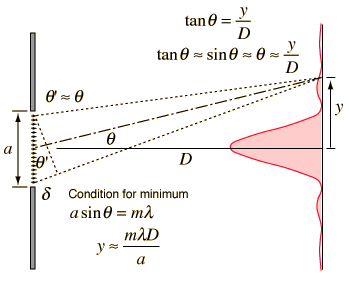
\includegraphics[width=.75\textwidth]{sinslit.png}
    \label{fig:fraunhofer}
\end{figure}

\end{document}